\documentclass[compress,red]{beamer}
\mode<presentation>
\setbeamertemplate{navigation symbols}{}

\usetheme{Warsaw}


%\hypersetup{pdfpagemode=FullScreen} % makes your presentation go automatically to full screen

% define your own colors:
\definecolor{Red}{rgb}{1,0,0}
\definecolor{Blue}{rgb}{0,0,1}
\definecolor{Green}{rgb}{0,1,0}
\definecolor{magenta}{rgb}{1,0,.6}
\definecolor{lightblue}{rgb}{0,.5,1}
\definecolor{lightpurple}{rgb}{.6,.4,1}
\definecolor{gold}{rgb}{.6,.5,0}
\definecolor{orange}{rgb}{1,0.4,0}
\definecolor{hotpink}{rgb}{1,0,0.5}
\definecolor{newcolor2}{rgb}{.5,.3,.5}
\definecolor{newcolor}{rgb}{0,.3,1}
\definecolor{newcolor3}{rgb}{1,0,.35}
\definecolor{darkgreen1}{rgb}{0, .35, 0}
\definecolor{darkgreen}{rgb}{0, .6, 0}
\definecolor{darkred}{rgb}{.75,0,0}

\xdefinecolor{olive}{cmyk}{0.64,0,0.95,0.4}
\xdefinecolor{purpleish}{cmyk}{0.75,0.75,0,0}


\useoutertheme[subsection=false]{smoothbars}


% include packages
\usepackage{subfigure}
\usepackage{multicol}
\usepackage{amsmath}
\usepackage{epsfig}
\usepackage{graphicx}
\usepackage[all,knot]{xy}
\xyoption{arc}
\usepackage{url}
\usepackage{multimedia}
\usepackage{hyperref}
\usepackage{helvet}
\usepackage[polish,english]{babel}
\usepackage[utf8]{inputenc}
\usepackage{multirow}
%%%%%%%%%%%%5
%\usepackage{geometry}
%\geometry{verbose,letterpaper}
%\usepackage{movie15}
%\usepackage{hyperref}
%%%%%%%

% greetings, introduce yourself


%  \includegraphics[height=5cm]{fig/WRlogo.ps}


\title[White Rabbit Specification\hspace{2em}\insertframenumber/ \inserttotalframenumber]
{White Rabbit Specification \\ version 2}

\institute{
$5^{th}$ White Rabbit Workshop \\ CERN
}
\author{
Maciej Lipi\'{n}ski %, T.W\l{}ostowski, J.Serrano, P.Alvarez
}
\date{September 19, 2011}



% \institute%[Universities of Somewhere and Elsewhere] % (optional, but mostly needed)
% {
%   \begin{center}
%     BE-CO-HT\\
%     CERN, Geneva,\\
%     Switzerland\\
%   \end{center}
% }

\pgfdeclareimage[height=0.6cm]{wr-logo}{../../figures/logo/WRlogo.ps}
\logo{\pgfuseimage{wr-logo}}
\AtBeginSection[]
% {
%   \begin{frame}<beamer>{Outline}
%     \tableofcontents[currentsection]
%   \end{frame}
% }

\begin{document}

\frame{\titlepage}
%%%%%%%%%%%%%%%%%%%%%%%%%%%%%%%%%%%%%%%%%%%%%%%%%%%%%%%%%%%%%%%%%%%%%%%%%%%%%%%%%%%%%%%%%%%%%%%%%%%%
\begin{frame}<beamer>{Outline}

    \tableofcontents %[currentsection]

\end{frame}
%%%%%%%%%%%%%%%%%%%%%%%%%%%%%%%%%%%%%%%%%%%%%%%%%%%%%%%%%%%%%%%%%%%%%%%%%%%%%%%%%%%%%%%%%%%%%%%%%%%%
\section{Introduction}
\subsection{}
%%%%%%%%%%%%%%%%%%%%%%%%%%%%%%%%%%%%%%%%%%%%%%%%%%%%%%%%%%%%%%%%%%%%%%%%%%%%%%%%%%%%%%%%%%%%%%%%%%%%
\begin{frame}{Time Distribution in White Rabbit}

  \begin{itemize}
    \item Synchronization with {\bf sub-ns} accuracy over fiber
    \item Combination of
	\begin{itemize}
	  \item Precision Time Protocol ({\bf PTP}) synchronization
	  \item Synchronous Ethernet ({\bf SyncE}) syntonization
	  \item Digital Dual-Mixer Time Difference ({\bf DDMTD}) phase detection
	\end{itemize}
%    \item Reliability-oriented.
    \item WR Link:
  \end{itemize}

  \begin{center}
  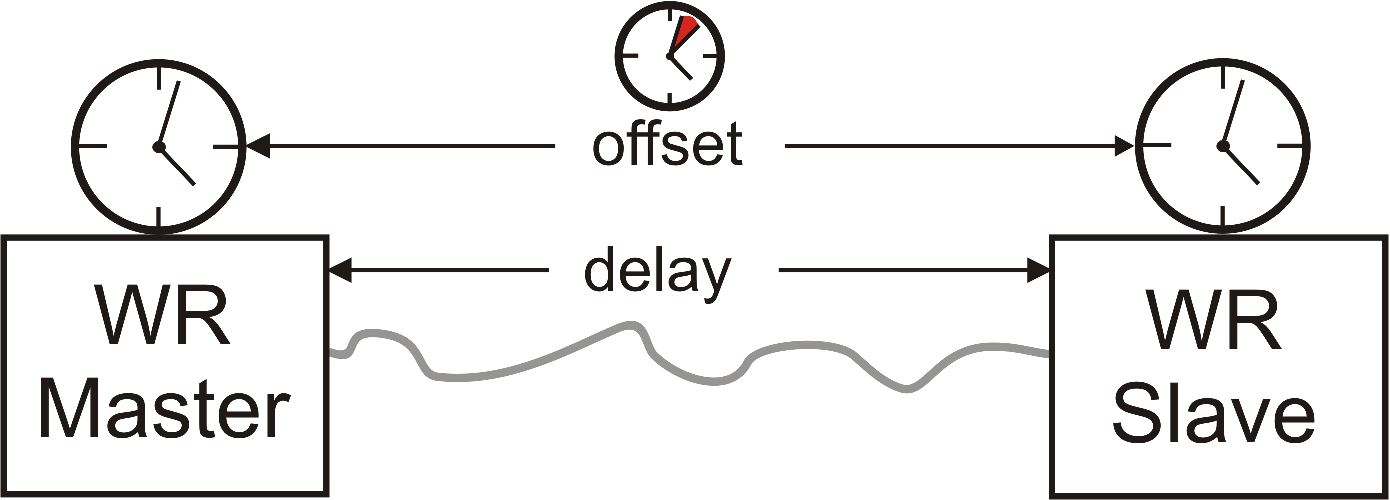
\includegraphics[height=3cm]{../../figures/protocol/wrLink.ps}
  \end{center}

\end{frame}
%%%%%%%%%%%%%%%%%%%%%%%%%%%%%%%%%%%%%%%%%%%%%%%%%%%%%%%%%%%%%%%%%%%%%%%%%%%%%%%%%%%%%%%%%%%%%%%%%%%%
% \subsection{}
%%%%%%%%%%%%%%%%%%%%%%%%%%%%%%%%%%%%%%%%%%%%%%%%%%%%%%%%%%%%%%%%%%%%%%%%%%%%%%%%%%%%%%%%%%%%%%%%%%%%
\begin{frame}{Time Distribution in White Rabbit}

\center A White Rabbit Network
  \begin{center}
  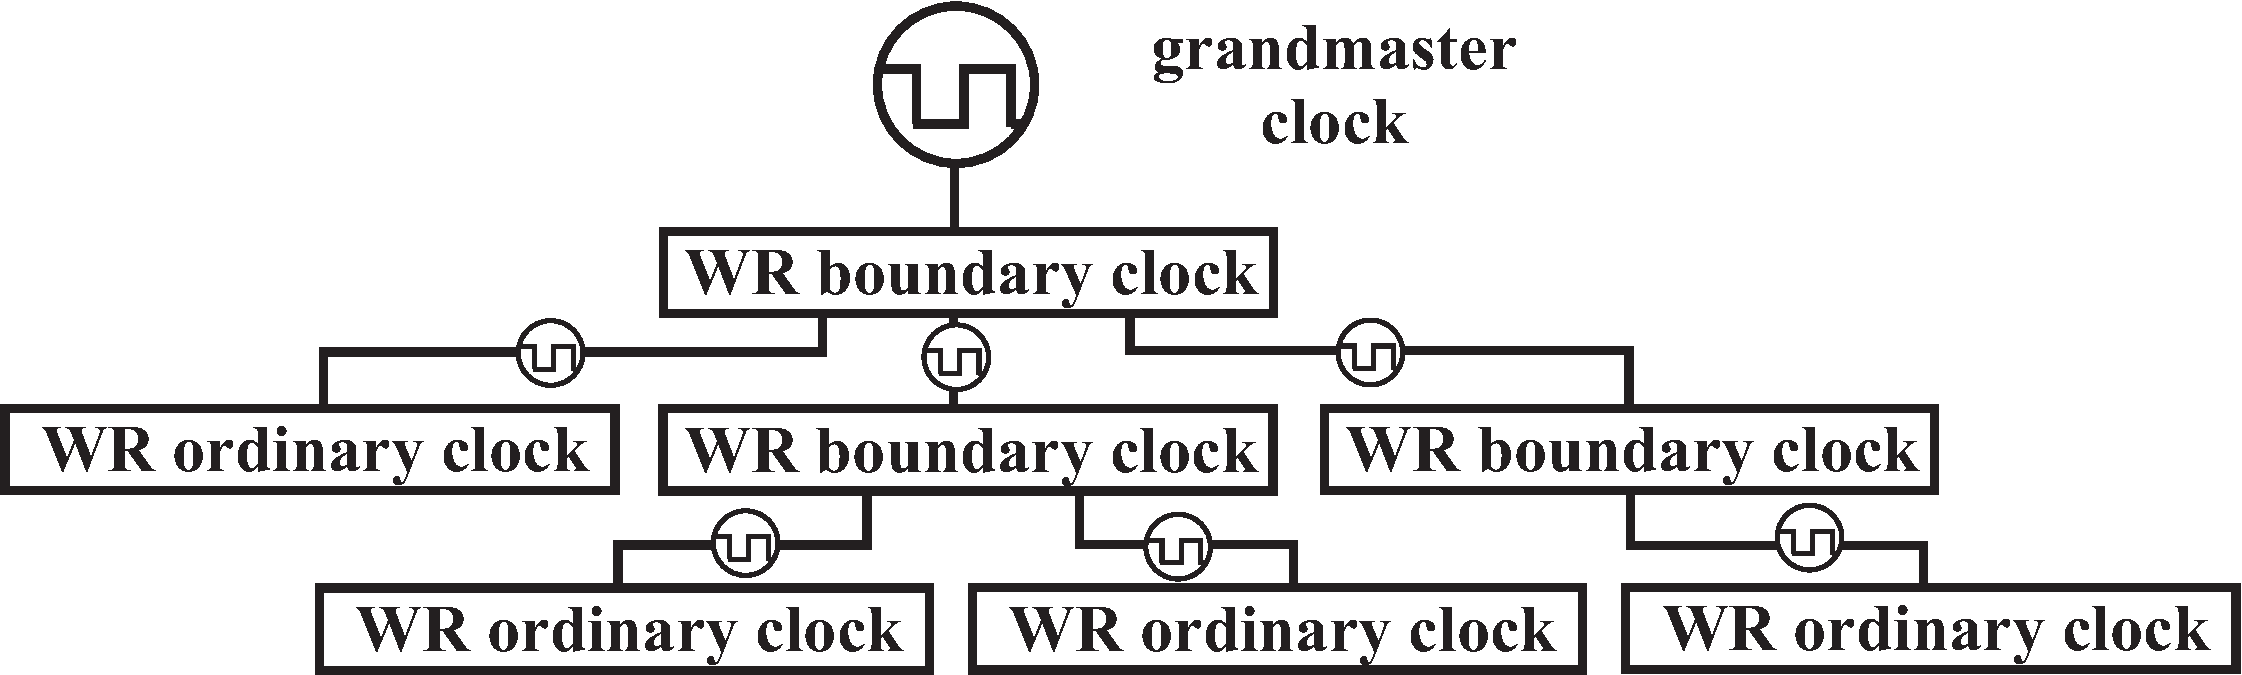
\includegraphics[width=11.5cm]{../../figures/network/wrTopology.eps}
  \end{center}
\end{frame}
%%%%%%%%%%%%%%%%%%%%%%%%%%%%%%%%%%%%%%%%%%%%%%%%%%%%%%%%%%%%%%%%%%%%%%%%%%%%%%%%%%%%%%%%%%%%%%%%%%%%
% \section{PTP}
% \subsection{}
\begin{frame}{Precision Time Protocol (PTP)}
%%%%%%%%%%%%%%%%%%%%%%%%%%%%%%%%%%%%%%%%%%%%%%%%%%%%%%%%%%%%%%%%%%%%%%%%%%%%%%%%%%%%%%%%%%%%%%%%%%%%
\begin{columns}[c]
\column{2.8in}

  \begin{itemize}
    \item IEEE1588-2008 standard
    \item packet-based protocol 
    \item synchronizes devices in distributed systems
    \item Best Master Clock (BMC) Algorithm -- defines the role PTP node 
  \end{itemize}

\column{1.5in}
    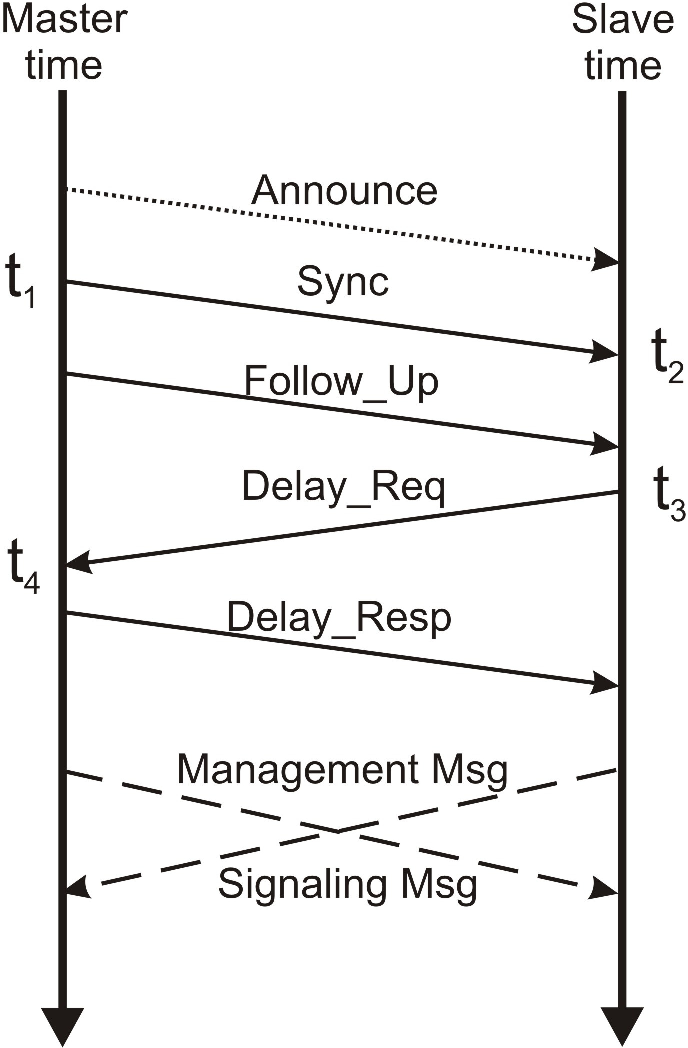
\includegraphics[height=5.5cm]{../../figures/protocol/ptpMSGs.ps} \\
    \small 
    one-way mean delay: \\
    $\mu = \frac{(t_{4}-t_{1}) - (t_{3}-t_{2})}{2}$ \\
    \small 
    $offset = t_{2} - (t_{1} + \mu)$
    
\end{columns}


\end{frame}
%%%%%%%%%%%%%%%%%%%%%%%%%%%%%%%%%%%%%%%%%%%%%%%%%%%%%%%%%%%%%%%%%%%%%%%%%%%%%%%%%%%%%%%%%%%%%%%%%%%%
% \subsection{}
%%%%%%%%%%%%%%%%%%%%%%%%%%%%%%%%%%%%%%%%%%%%%%%%%%%%%%%%%%%%%%%%%%%%%%%%%%%%%%%%%%%%%%%%%%%%%%%%%%%%
\begin{frame}{Why not standard PTP?}

  \resizebox{11cm}{!} 
  {
    \begin{tabular}{ r c l }
  {\bf What are the issues...} 	& {\bf and}      & {\bf ... how we address them}  \\
				&     		 &        \\
      PTP-base		 	& \multirow{2}{*}{$\Rightarrow$}  & \multirow{2}{*}{SyncE }\\
      syntonization	        &      		 &        \\
				&      		 &        			\\
      limited             	&\multirow{2}{*}{$\Rightarrow$}  	 & SyncE \\
      precision and resolution  &      		 & DDTMD phase detection\\
				&    		 &        \\
			        &      		 & SyncE  \\
      unknown link asymmetry    & $\Rightarrow$  & DDTMD phase detection \\
				&      		 & WR Link Delay Model \\
				&      		 &        \\
      \multicolumn{3}{c}{WR extension to PTP ({\bf WRPTP}) for } \\
      \multicolumn{3}{c}{extra data exchange and logic} \\
    \end{tabular}
  }
\end{frame}

%%%%%%%%%%%%%%%%%%%%%%%%%%%%%%%%%%%%%%%%%%%%%%%%%%%%%%%%%%%%%%%%%%%%%%%%%%%%%%%%%%%%%%%%%%%%%%%%%%%%
\section{Link Delay Model}
\subsection{}
%%%%%%%%%%%%%%%%%%%%%%%%%%%%%%%%%%%%%%%%%%%%%%%%%%%%%%%%%%%%%%%%%%%%%%%%%%%%%%%%%%%%%%%%%%%%%%%%%%%%
\begin{frame}{Link Delay Model}

  \begin{align}
    \nonumber delay_{ms} &= \Delta_{tx_m} + \delta_{ms} + \Delta_{rx_s} \\
    \nonumber delay_{sm} &= \Delta_{tx_s} + \delta_{sm} + \Delta_{rx_m}
  \end{align}

   \vspace{0.2cm}

  \begin{center}
  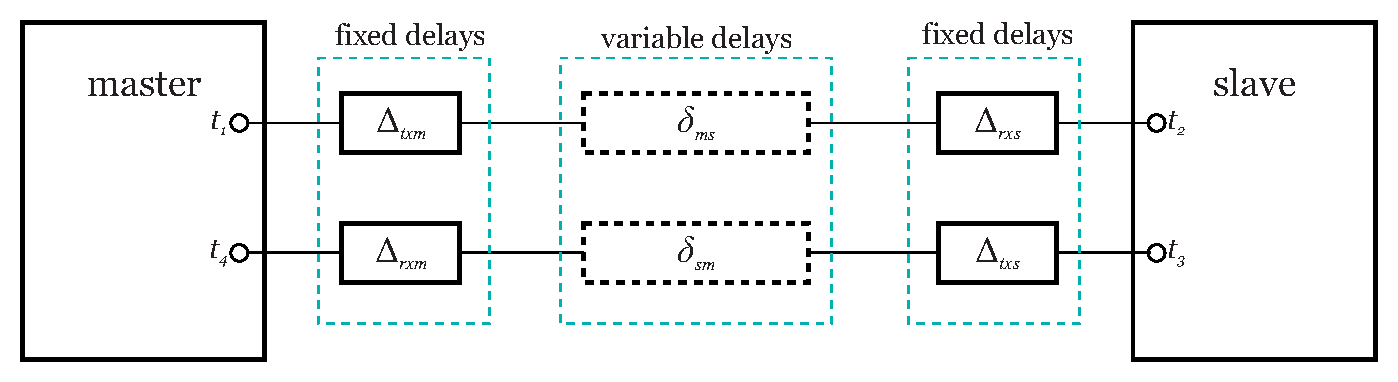
\includegraphics[height=2.5cm]{../../figures/protocol/delaymodel.eps}
  \end{center}

\begin{columns}[c]
  \column{2.8in}

    \begin{center}
      \textbf{Relative Delay Coefficient ($\alpha$)} \\
      for 1000base-X over a Single-mode Optical Fibre
    \end{center}

  \column{1.5in}
    \begin{center}
      \begin{equation}
      \nonumber \delta_{ms} = (1 + \alpha) \, \delta_{sm}
      \end{equation}
    \end{center}
    \vspace{0.5cm}
\end{columns}
  

\end{frame}
%%%%%%%%%%%%%%%%%%%%%%%%%%%%%%%%%%%%%%%%%%%%%%%%%%%%%%%%%%%%%%%%%%%%%%%%%%%%%%%%%%%%%%%%%%%%%%%%%%%%
% \subsection{}
%%%%%%%%%%%%%%%%%%%%%%%%%%%%%%%%%%%%%%%%%%%%%%%%%%%%%%%%%%%%%%%%%%%%%%%%%%%%%%%%%%%%%%%%%%%%%%%%%%%%
\begin{frame}{Link Delay Model: fiber optic solution}

  \begin{center}
  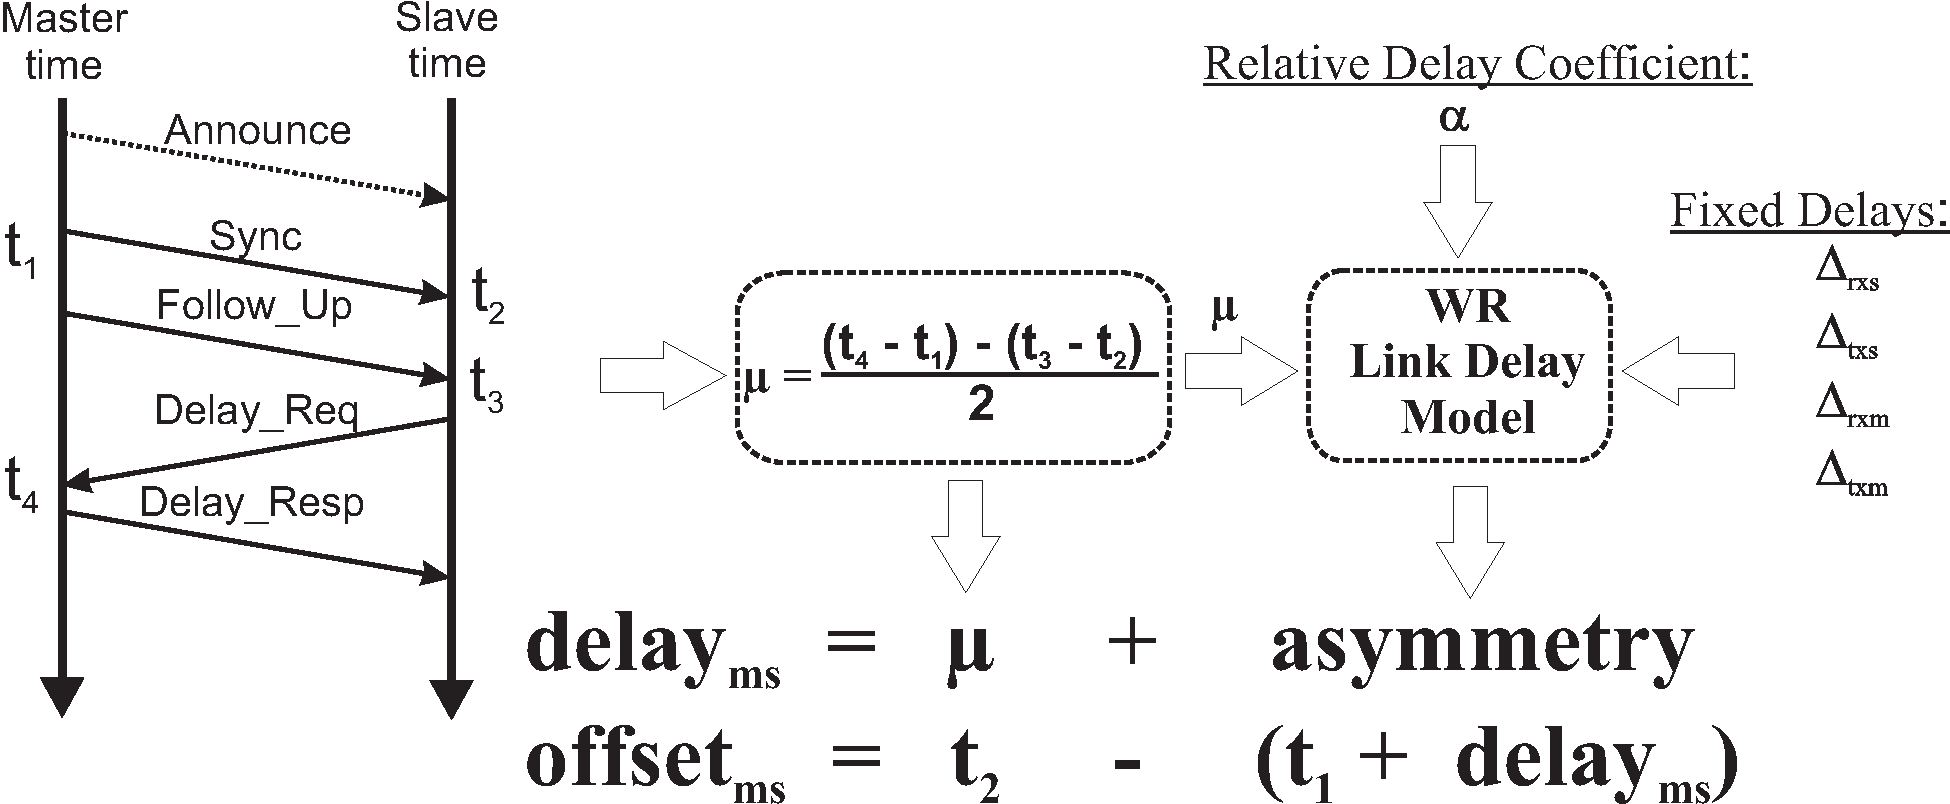
\includegraphics[height=4cm]{../../figures/protocol/wrLinkModel.eps}
  \end{center}

  \begin{columns}[c]
  \column{1.5in}

    \begin{center}
      \textbf{Solution for Ethernet over a Single-mode Optical Fiber}
    \end{center}    

  \column{2.7in}

    \begin{equation}
      \nonumber asymmetry = \Delta_{tx_m} + \Delta_{rx_s} - \frac{\Delta - \alpha \mu + \alpha \Delta}{2 + \alpha}
    \end{equation}

  \end{columns}

\end{frame}
% %%%%%%%%%%%%%%%%%%%%%%%%%%%%%%%%%%%%%%%%%%%%%%%%%%%%%%%%%%%%%%%%%%%%%%%%%%%%%%%%%%%%%%%%%%%%%%%%%%%%
% \section{}
% \subsection{}
% %%%%%%%%%%%%%%%%%%%%%%%%%%%%%%%%%%%%%%%%%%%%%%%%%%%%%%%%%%%%%%%%%%%%%%%%%%%%%%%%%%%%%%%%%%%%%%%%%%%%
% \begin{frame}{Overview of White Rabbit Distribution}
% 
% fill in
% 
% \end{frame}
%%%%%%%%%%%%%%%%%%%%%%%%%%%%%%%%%%%%%%%%%%%%%%%%%%%%%%%%%%%%%%%%%%%%%%%%%%%%%%%%%%%%%%%%%%%%%%%%%%%%
\section{H/W for WR}
\subsection{}
%%%%%%%%%%%%%%%%%%%%%%%%%%%%%%%%%%%%%%%%%%%%%%%%%%%%%%%%%%%%%%%%%%%%%%%%%%%%%%%%%%%%%%%%%%%%%%%%%%%%
% \begin{frame}{HW4WR}
% 
%   \begin{itemize}
%     \item Fine Delay Measurement,
%     \item Clock Recovery System,
%     \item Fixed Delays Measurement.
%   \end{itemize}
% 
% 
% \end{frame}
%%%%%%%%%%%%%%%%%%%%%%%%%%%%%%%%%%%%%%%%%%%%%%%%%%%%%%%%%%%%%%%%%%%%%%%%%%%%%%%%%%%%%%%%%%%%%%%%%%%%
% \subsection{}
%%%%%%%%%%%%%%%%%%%%%%%%%%%%%%%%%%%%%%%%%%%%%%%%%%%%%%%%%%%%%%%%%%%%%%%%%%%%%%%%%%%%%%%%%%%%%%%%%%%%
\setbeamertemplate{background}{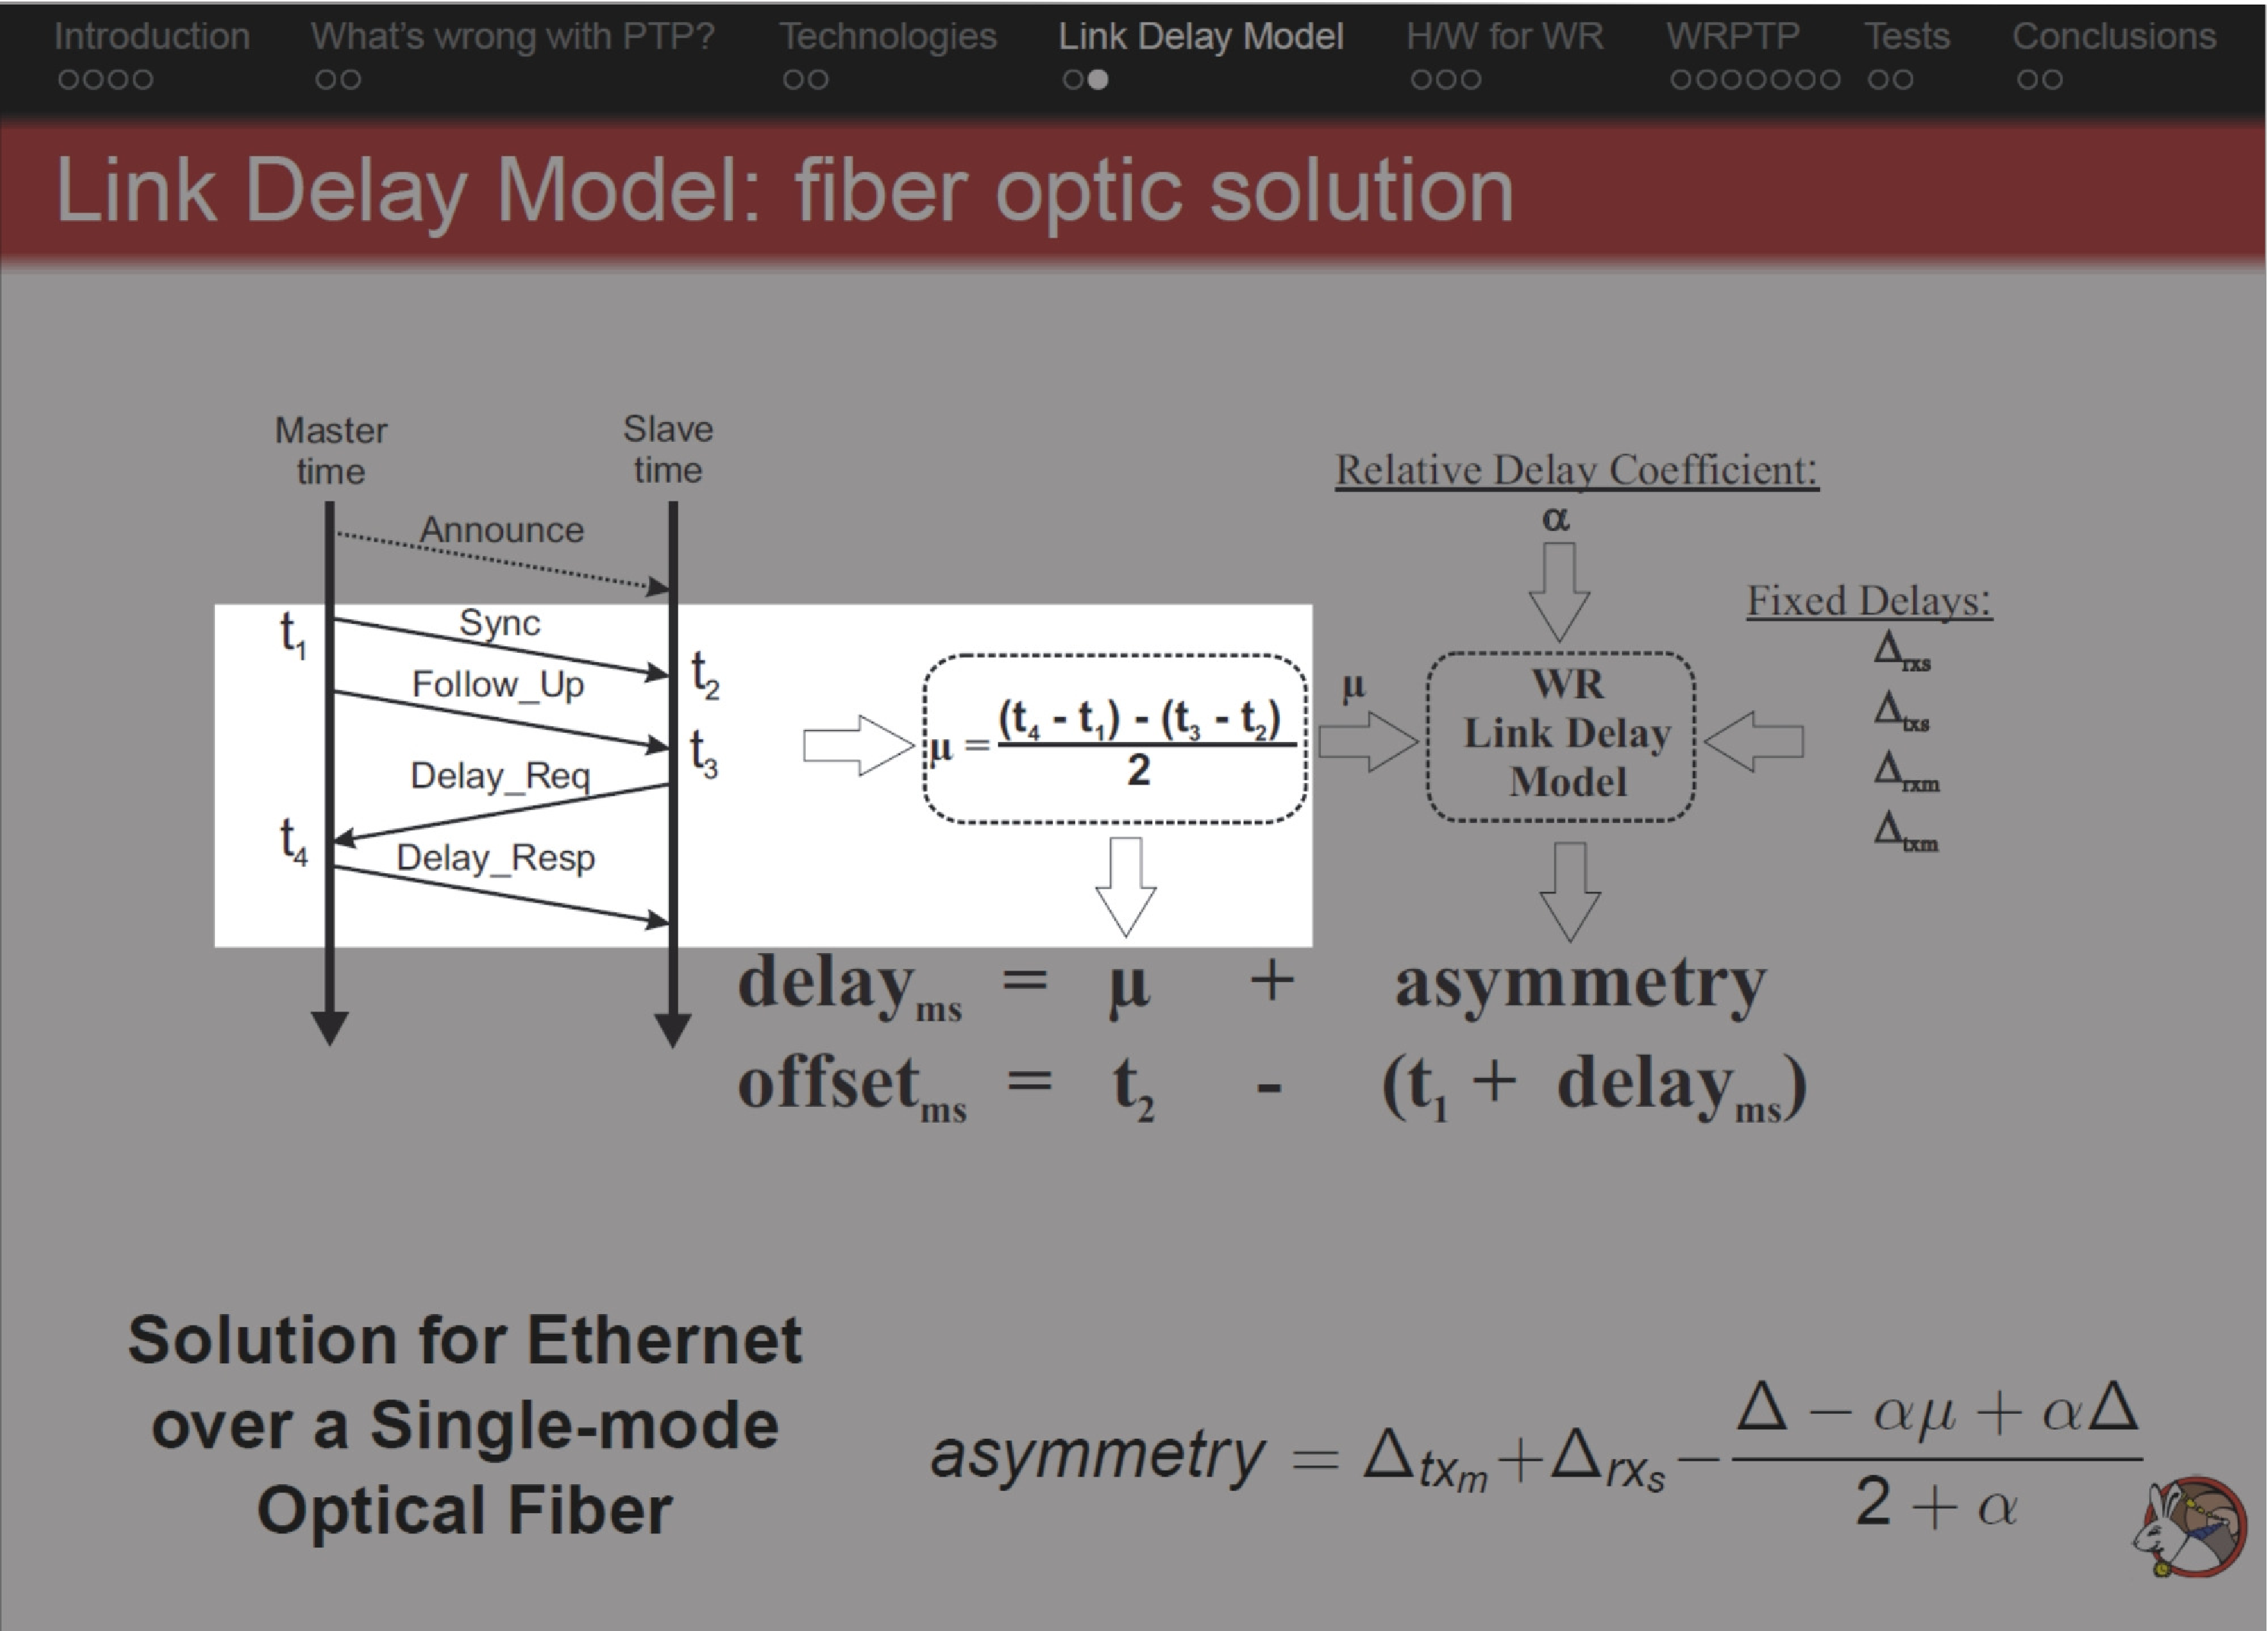
\includegraphics[width=\paperwidth]{../../figures/protocol/wrLinkModel-fdm2.ps}} 
\logo{}
\begin{frame}{Fine Delay Measurement}

%background

\end{frame}
\setbeamertemplate{background}{} 
\logo{\pgfuseimage{wr-logo}}
%%%%%%%%%%%%%%%%%%%%%%%%%%%%%%%%%%%%%%%%%%%%%%%%%%%%%%%%%%%%%%%%%%%%%%%%%%%%%%%%%%%%%%%%%%%%%%%%%%%%
%\subsection{}
%%%%%%%%%%%%%%%%%%%%%%%%%%%%%%%%%%%%%%%%%%%%%%%%%%%%%%%%%%%%%%%%%%%%%%%%%%%%%%%%%%%%%%%%%%%%%%%%%%%%
\begin{frame}{Fine Delay Measurement}

  \begin{center}
  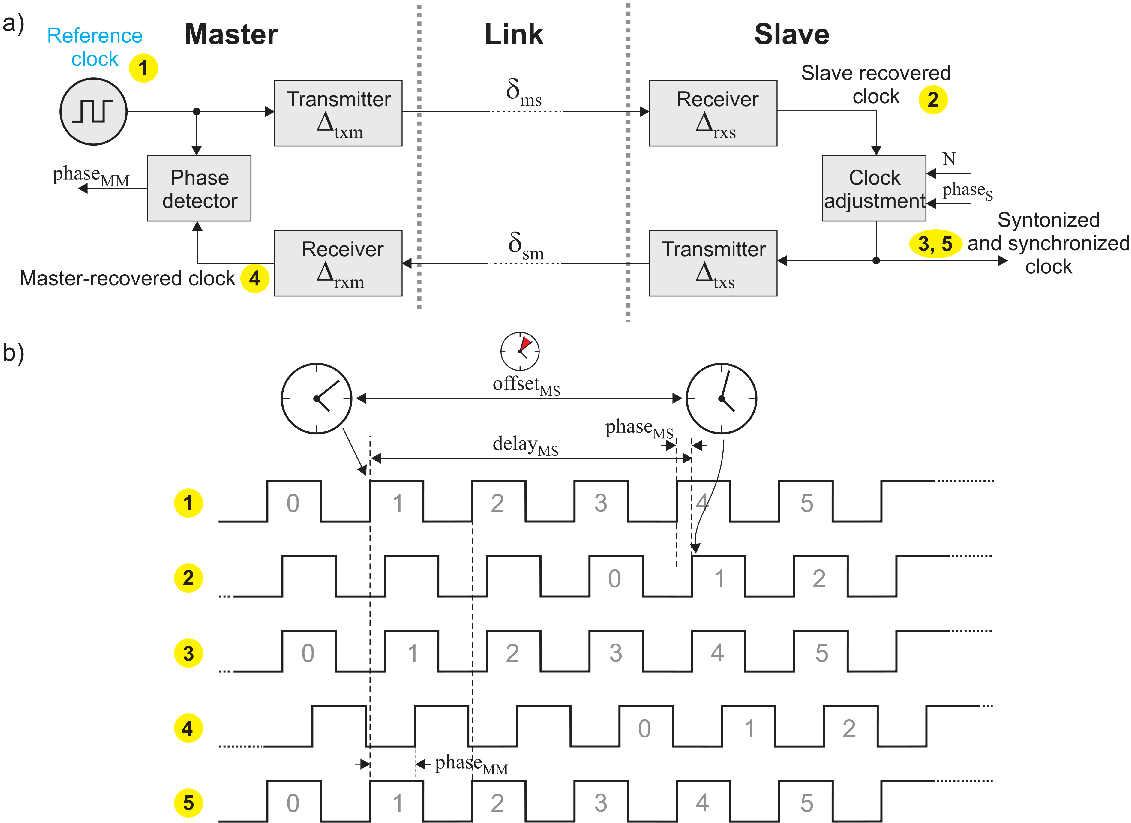
\includegraphics[width=10.0cm]{../../figures/protocol/link_model.eps}
  \end{center}

\end{frame}

%%%%%%%%%%%%%%%%%%%%%%%%%%%%%%%%%%%%%%%%%%%%%%%%%%%%%%%%%%%%%%%%%%%%%%%%%%%%%%%%%%%%%%%%%%%%%%%%%%%%
%\subsection{}
%%%%%%%%%%%%%%%%%%%%%%%%%%%%%%%%%%%%%%%%%%%%%%%%%%%%%%%%%%%%%%%%%%%%%%%%%%%%%%%%%%%%%%%%%%%%%%%%%%%%
\setbeamertemplate{background}{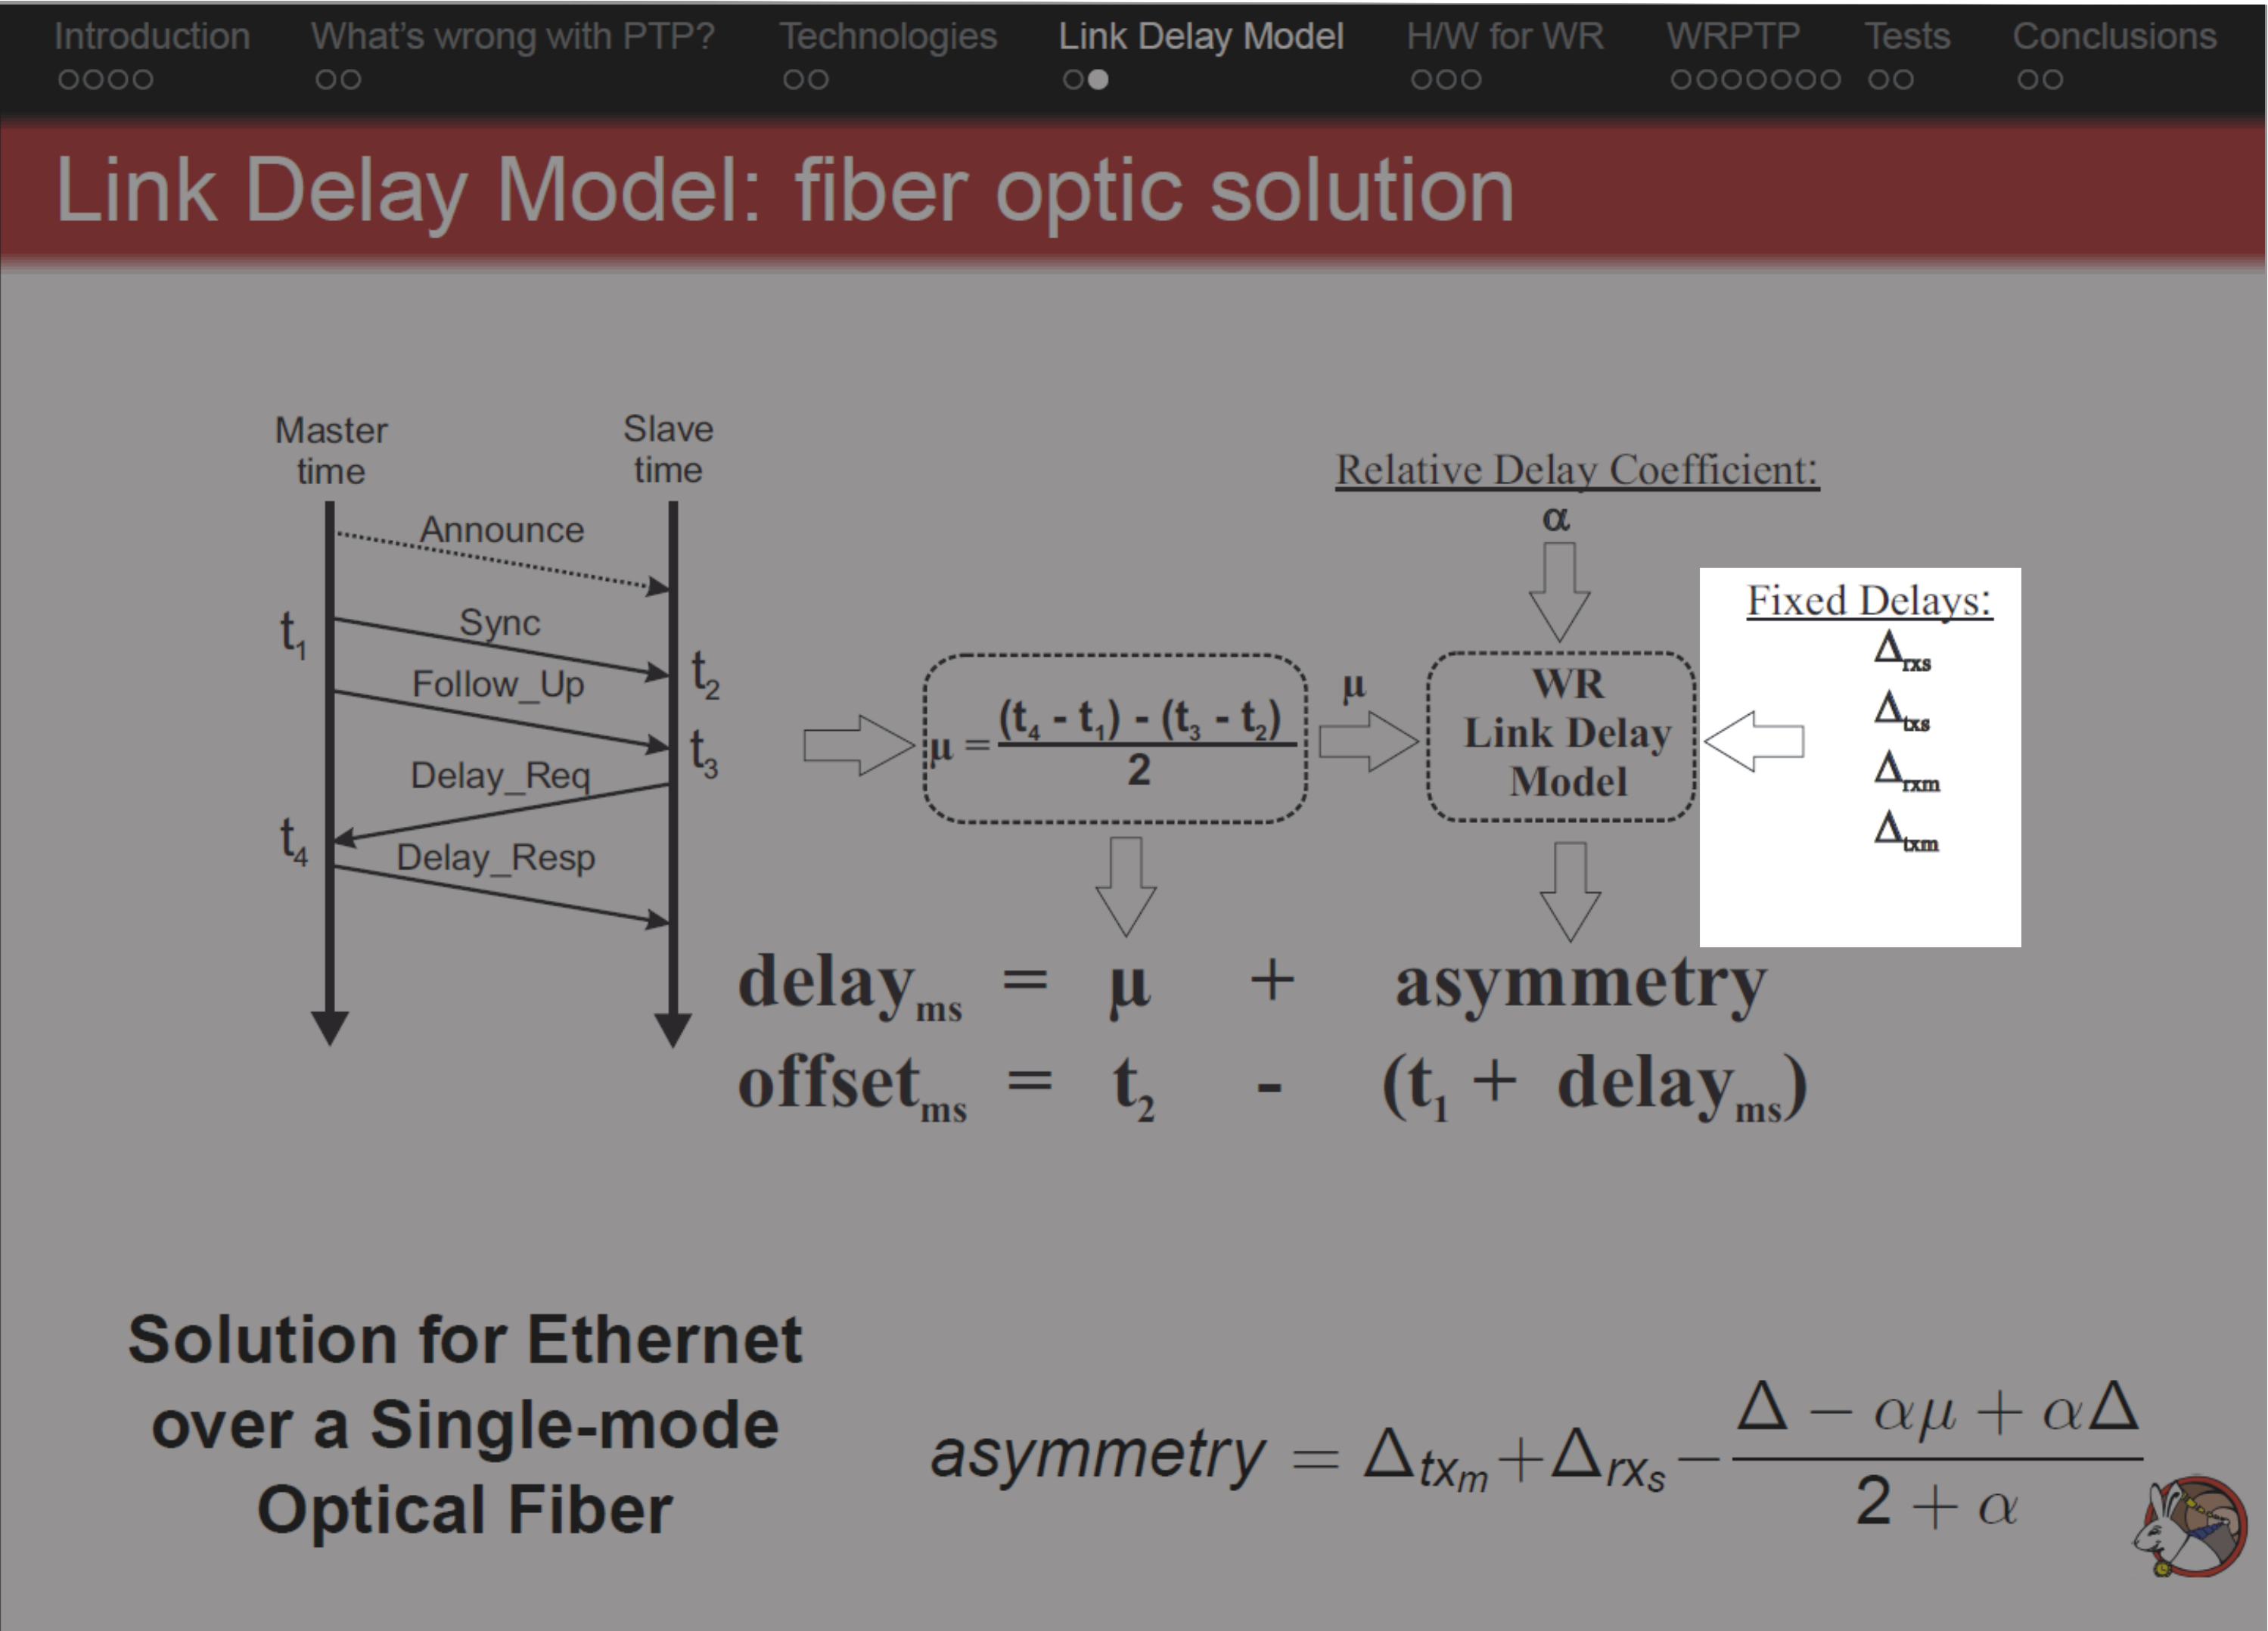
\includegraphics[width=\paperwidth]{../../figures/protocol/wrLinkModel-fd.ps}} 
\logo{}
\begin{frame}{Fixed Delays Measurement}

%background

\end{frame}
\setbeamertemplate{background}{} 
\logo{\pgfuseimage{wr-logo}}
%%%%%%%%%%%%%%%%%%%%%%%%%%%%%%%%%%%%%%%%%%%%%%%%%%%%%%%%%%%%%%%%%%%%%%%%%%%%%%%%%%%%%%%%%%%%%%%%%%%%
%\subsection{}
%%%%%%%%%%%%%%%%%%%%%%%%%%%%%%%%%%%%%%%%%%%%%%%%%%%%%%%%%%%%%%%%%%%%%%%%%%%%%%%%%%%%%%%%%%%%%%%%%%%%
\begin{frame}{Fixed Delays Measurement}

  \begin{center}
  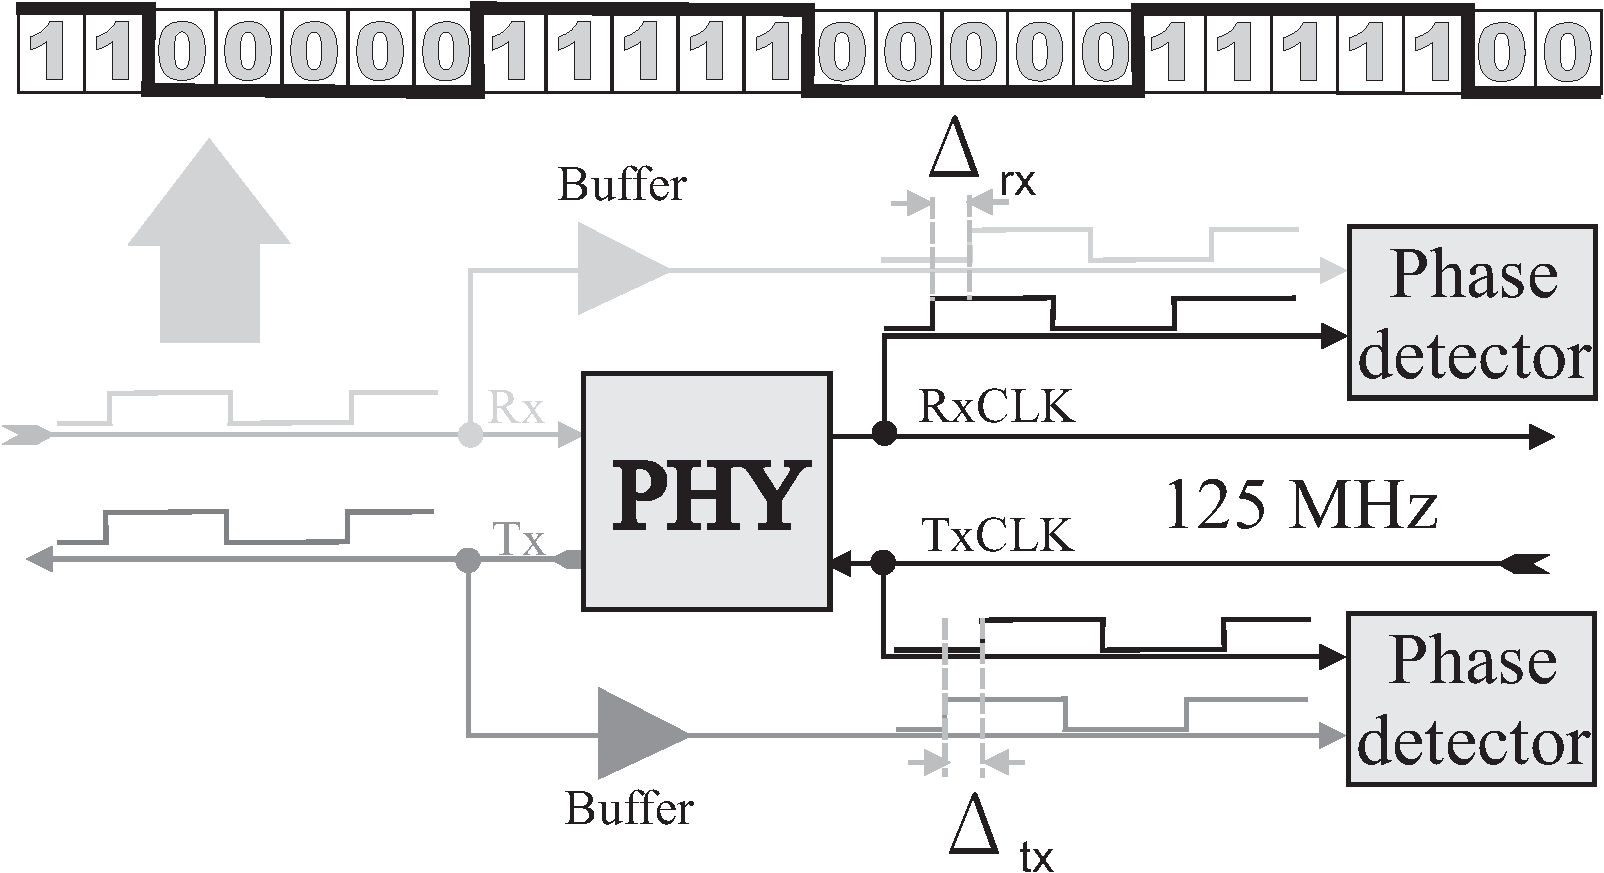
\includegraphics[width=10.0cm]{../../figures/misc/calibration.eps}
  \end{center}

\end{frame}
%%%%%%%%%%%%%%%%%%%%%%%%%%%%%%%%%%%%%%%%%%%%%%%%%%%%%%%%%%%%%%%%%%%%%%%%%%%%%%%%%%%%%%%%%%%%%%%%%%%%
\section{WRPTP}
\subsection{}
%%%%%%%%%%%%%%%%%%%%%%%%%%%%%%%%%%%%%%%%%%%%%%%%%%%%%%%%%%%%%%%%%%%%%%%%%%%%%%%%%%%%%%%%%%%%%%%%%%%%
\begin{frame}{White Rabbit extension to PTP (WRPTP)}

  \begin{itemize}
    \item WR-peers recognition
    \item Calibration
    \item Exchange of WR-data
    \item Support of redundancy
  \end{itemize}

\end{frame}
% we need to exchange some extra WR data in order to recognize WR peers (syncE),
% the exchange of data is also needed to perform calibration, where also some extra logic is needed
% and finaly to exchange the WR parameters. Finally, the support of time-source redundancy by 
% the standard PTP is not enough for WR, so we needed to change this as well
%%%%%%%%%%%%%%%%%%%%%%%%%%%%%%%%%%%%%%%%%%%%%%%%%%%%%%%%%%%%%%%%%%%%%%%%%%%%%%%%%%%%%%%%%%%%%%%%%%%%
% \section{WRPTP}
%\subsection{}
%%%%%%%%%%%%%%%%%%%%%%%%%%%%%%%%%%%%%%%%%%%%%%%%%%%%%%%%%%%%%%%%%%%%%%%%%%%%%%%%%%%%%%%%%%%%%%%%%%%%
\begin{frame}{Exchange of WR-data}

  \begin{columns}[c]
  \column{.5\textwidth} 

    \begin{center}
    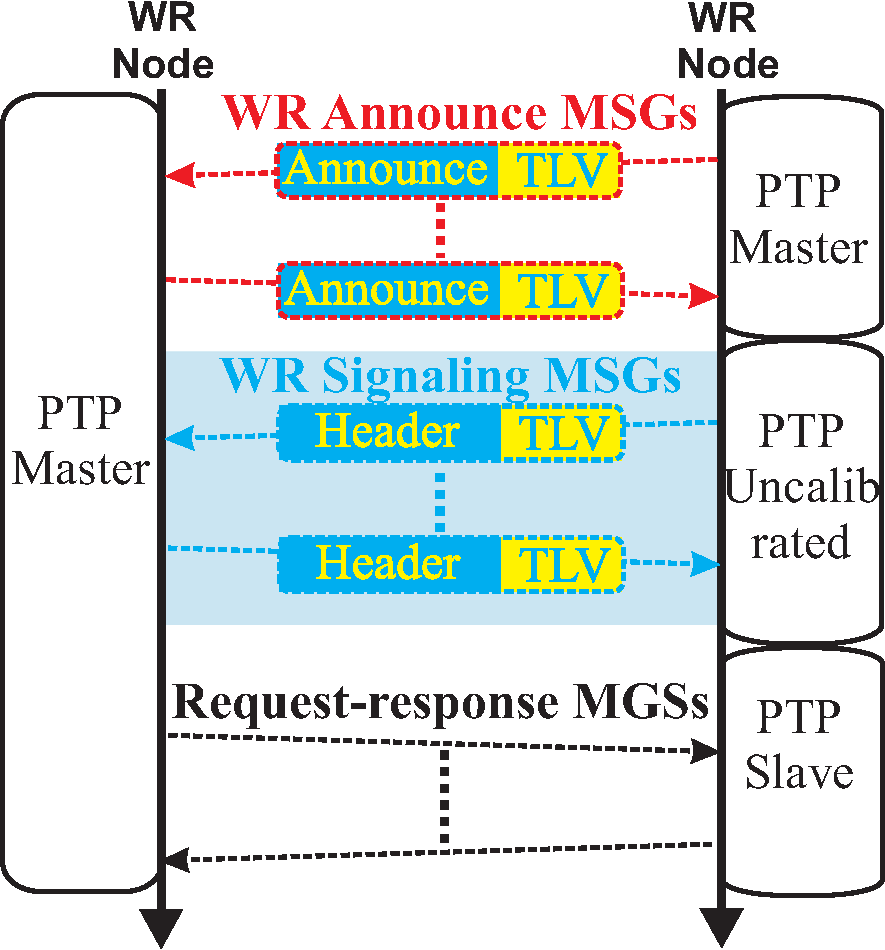
\includegraphics[width=5.5cm]{../../figures/protocol/WR-peer_recognision-1.eps}
    \end{center}

  \column{.5\textwidth}

      \begin{itemize}
	\item WR Type-Length-Value (WR TLV):
	  \begin{itemize}
	    \item ORGANIZATION\_EXT
	    \item CERN's OUI
	  \end{itemize}
 	\vspace{0.5cm}
	\item WR data stored:
	  \begin{itemize}
	    \item Additional Fields in PTP Data Sets
	    \item backupParentDS
	  \end{itemize}
% 	\vspace{0.5cm}
% 	\item WR data exchange by:
% 	  \begin{itemize}
% 	    \item suffixing Announce Messages
% 	    \item creating WR Signaling Messages
% 	  \end{itemize}
      \end{itemize}

  \end{columns}


\end{frame}
%%%%%%%%%%%%%%%%%%%%%%%%%%%%%%%%%%%%%%%%%%%%%%%%%%%%%%%%%%%%%%%%%%%%%%%%%%%%%%%%%%%%%%%%%%%%%%%%%%%%
% \subsection{}
%%%%%%%%%%%%%%%%%%%%%%%%%%%%%%%%%%%%%%%%%%%%%%%%%%%%%%%%%%%%%%%%%%%%%%%%%%%%%%%%%%%%%%%%%%%%%%%%%%%%
\begin{frame}{WR-peer recognition}

  \begin{columns}[c]
  \column{.5\textwidth} 

    \begin{center}
    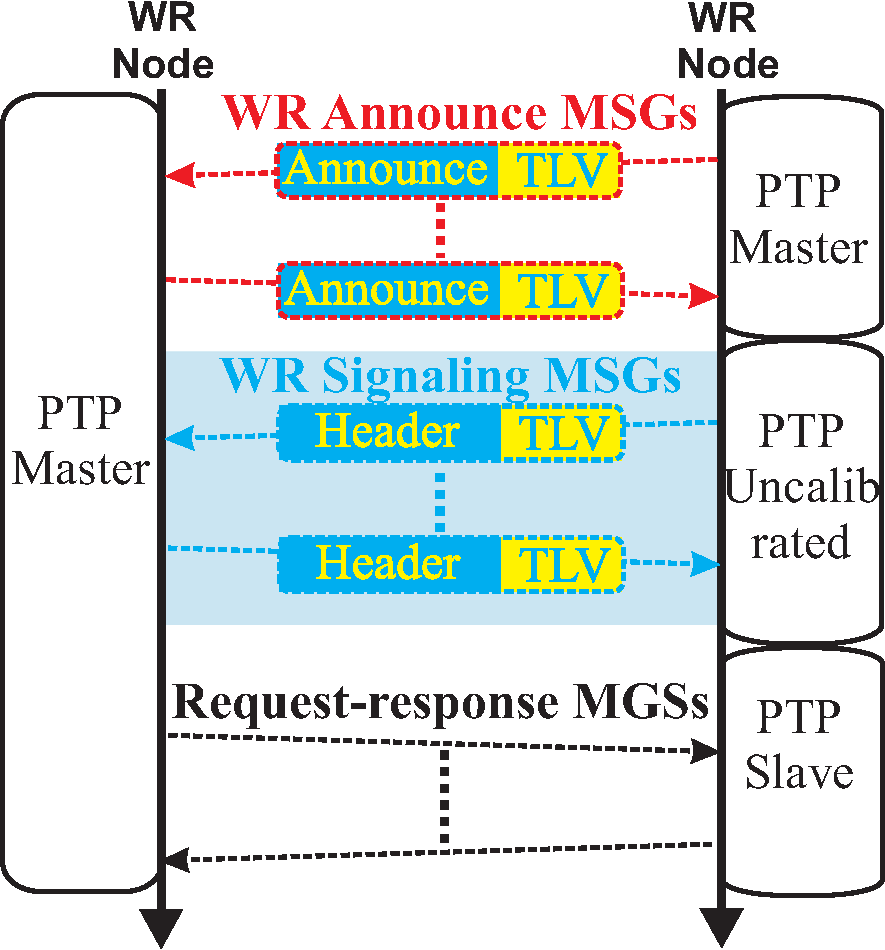
\includegraphics[width=5.5cm]{../../figures/protocol/WR-peer_recognision-1.eps}
    \end{center}

  \column{.5\textwidth}

    \begin{center}
    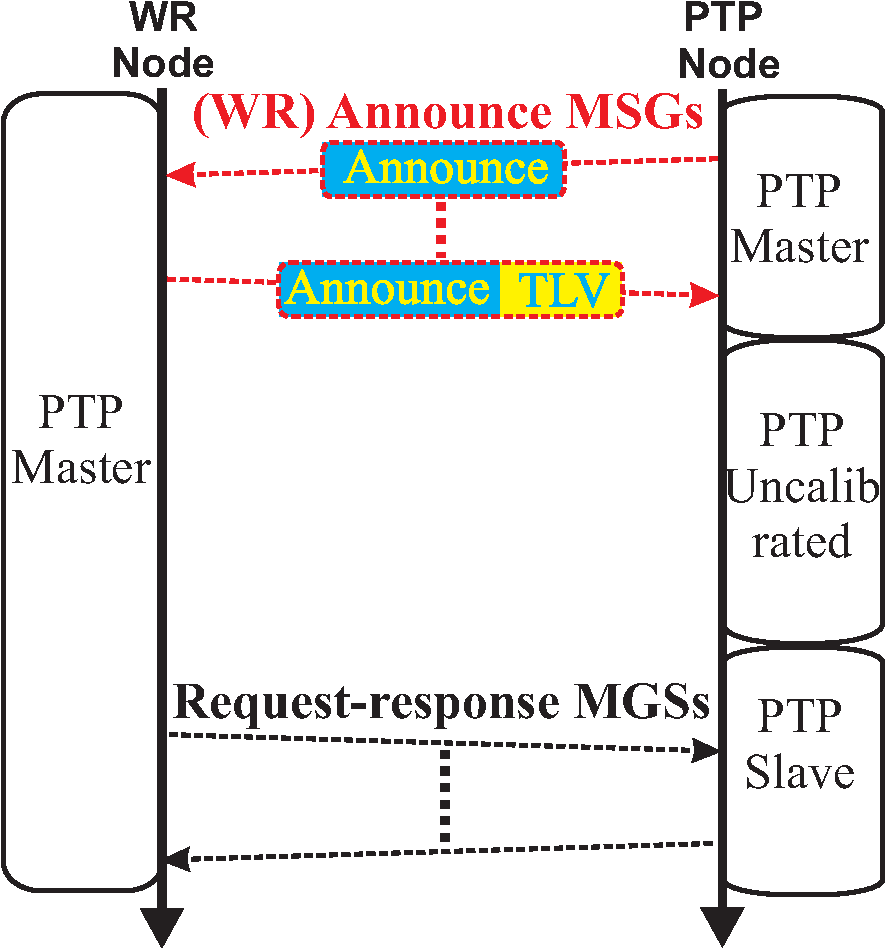
\includegraphics[width=5.5cm]{../../figures/protocol/WR-peer_recognision-2.eps}
    \end{center}

  \end{columns}

\end{frame}
%%%%%%%%%%%%%%%%%%%%%%%%%%%%%%%%%%%%%%%%%%%%%%%%%%%%%%%%%%%%%%%%%%%%%%%%%%%%%%%%%%%%%%%%%%%%%%%%%%%%
% \subsection{}
%%%%%%%%%%%%%%%%%%%%%%%%%%%%%%%%%%%%%%%%%%%%%%%%%%%%%%%%%%%%%%%%%%%%%%%%%%%%%%%%%%%%%%%%%%%%%%%%%%%%
\begin{frame}{WR Link Setup }

  \begin{columns}[c]
  \column{.5\textwidth} 

      \begin{center}
      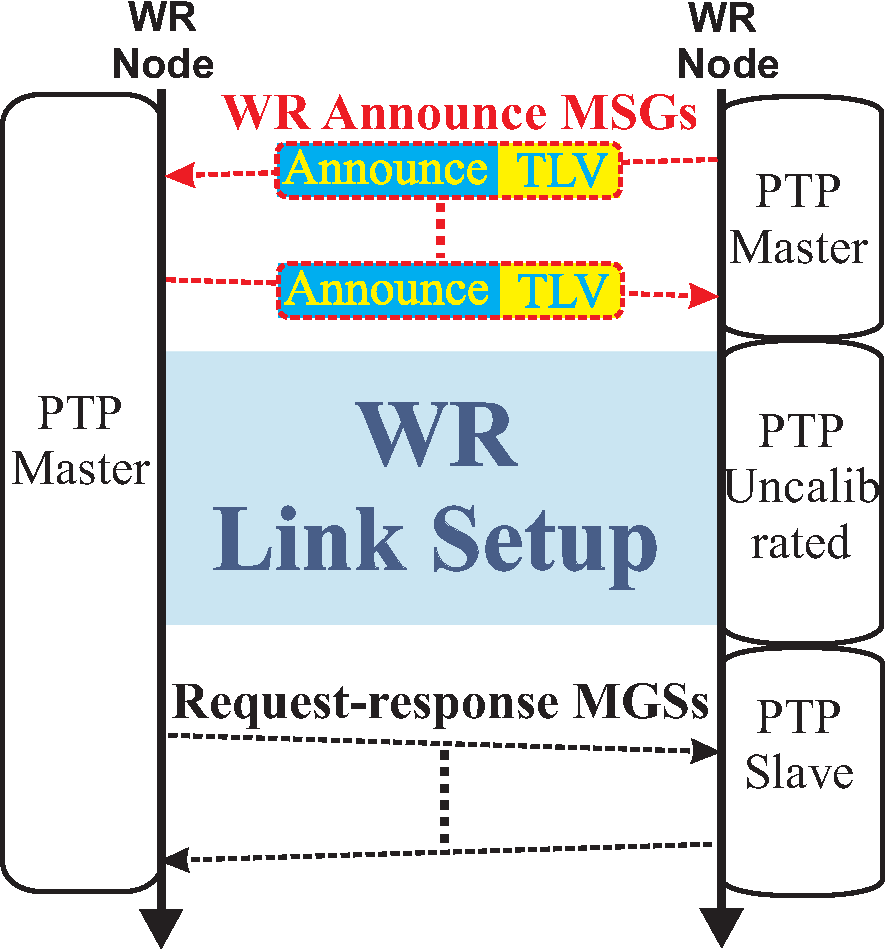
\includegraphics[width=5.5cm]{../../figures/protocol/wrLinkSetup.eps}
      \end{center}


  \column{.5\textwidth} 

      \begin{itemize}
	\item Frequency locking
	\item Calibration
	\item Exchange of WR-parameters
	\item WR Finite State Machine (FSM)
	\item WR Signaling Messages
      \end{itemize}

  \end{columns}

\end{frame}
%%%%%%%%%%%%%%%%%%%%%%%%%%%%%%%%%%%%%%%%%%%%%%%%%%%%%%%%%%%%%%%%%%%%%%%%%%%%%%%%%%%%%%%%%%%%%%%%%%%%
%\subsection{}
%%%%%%%%%%%%%%%%%%%%%%%%%%%%%%%%%%%%%%%%%%%%%%%%%%%%%%%%%%%%%%%%%%%%%%%%%%%%%%%%%%%%%%%%%%%%%%%%%%%%
\begin{frame}{WR Link Setup}

      \begin{center}
      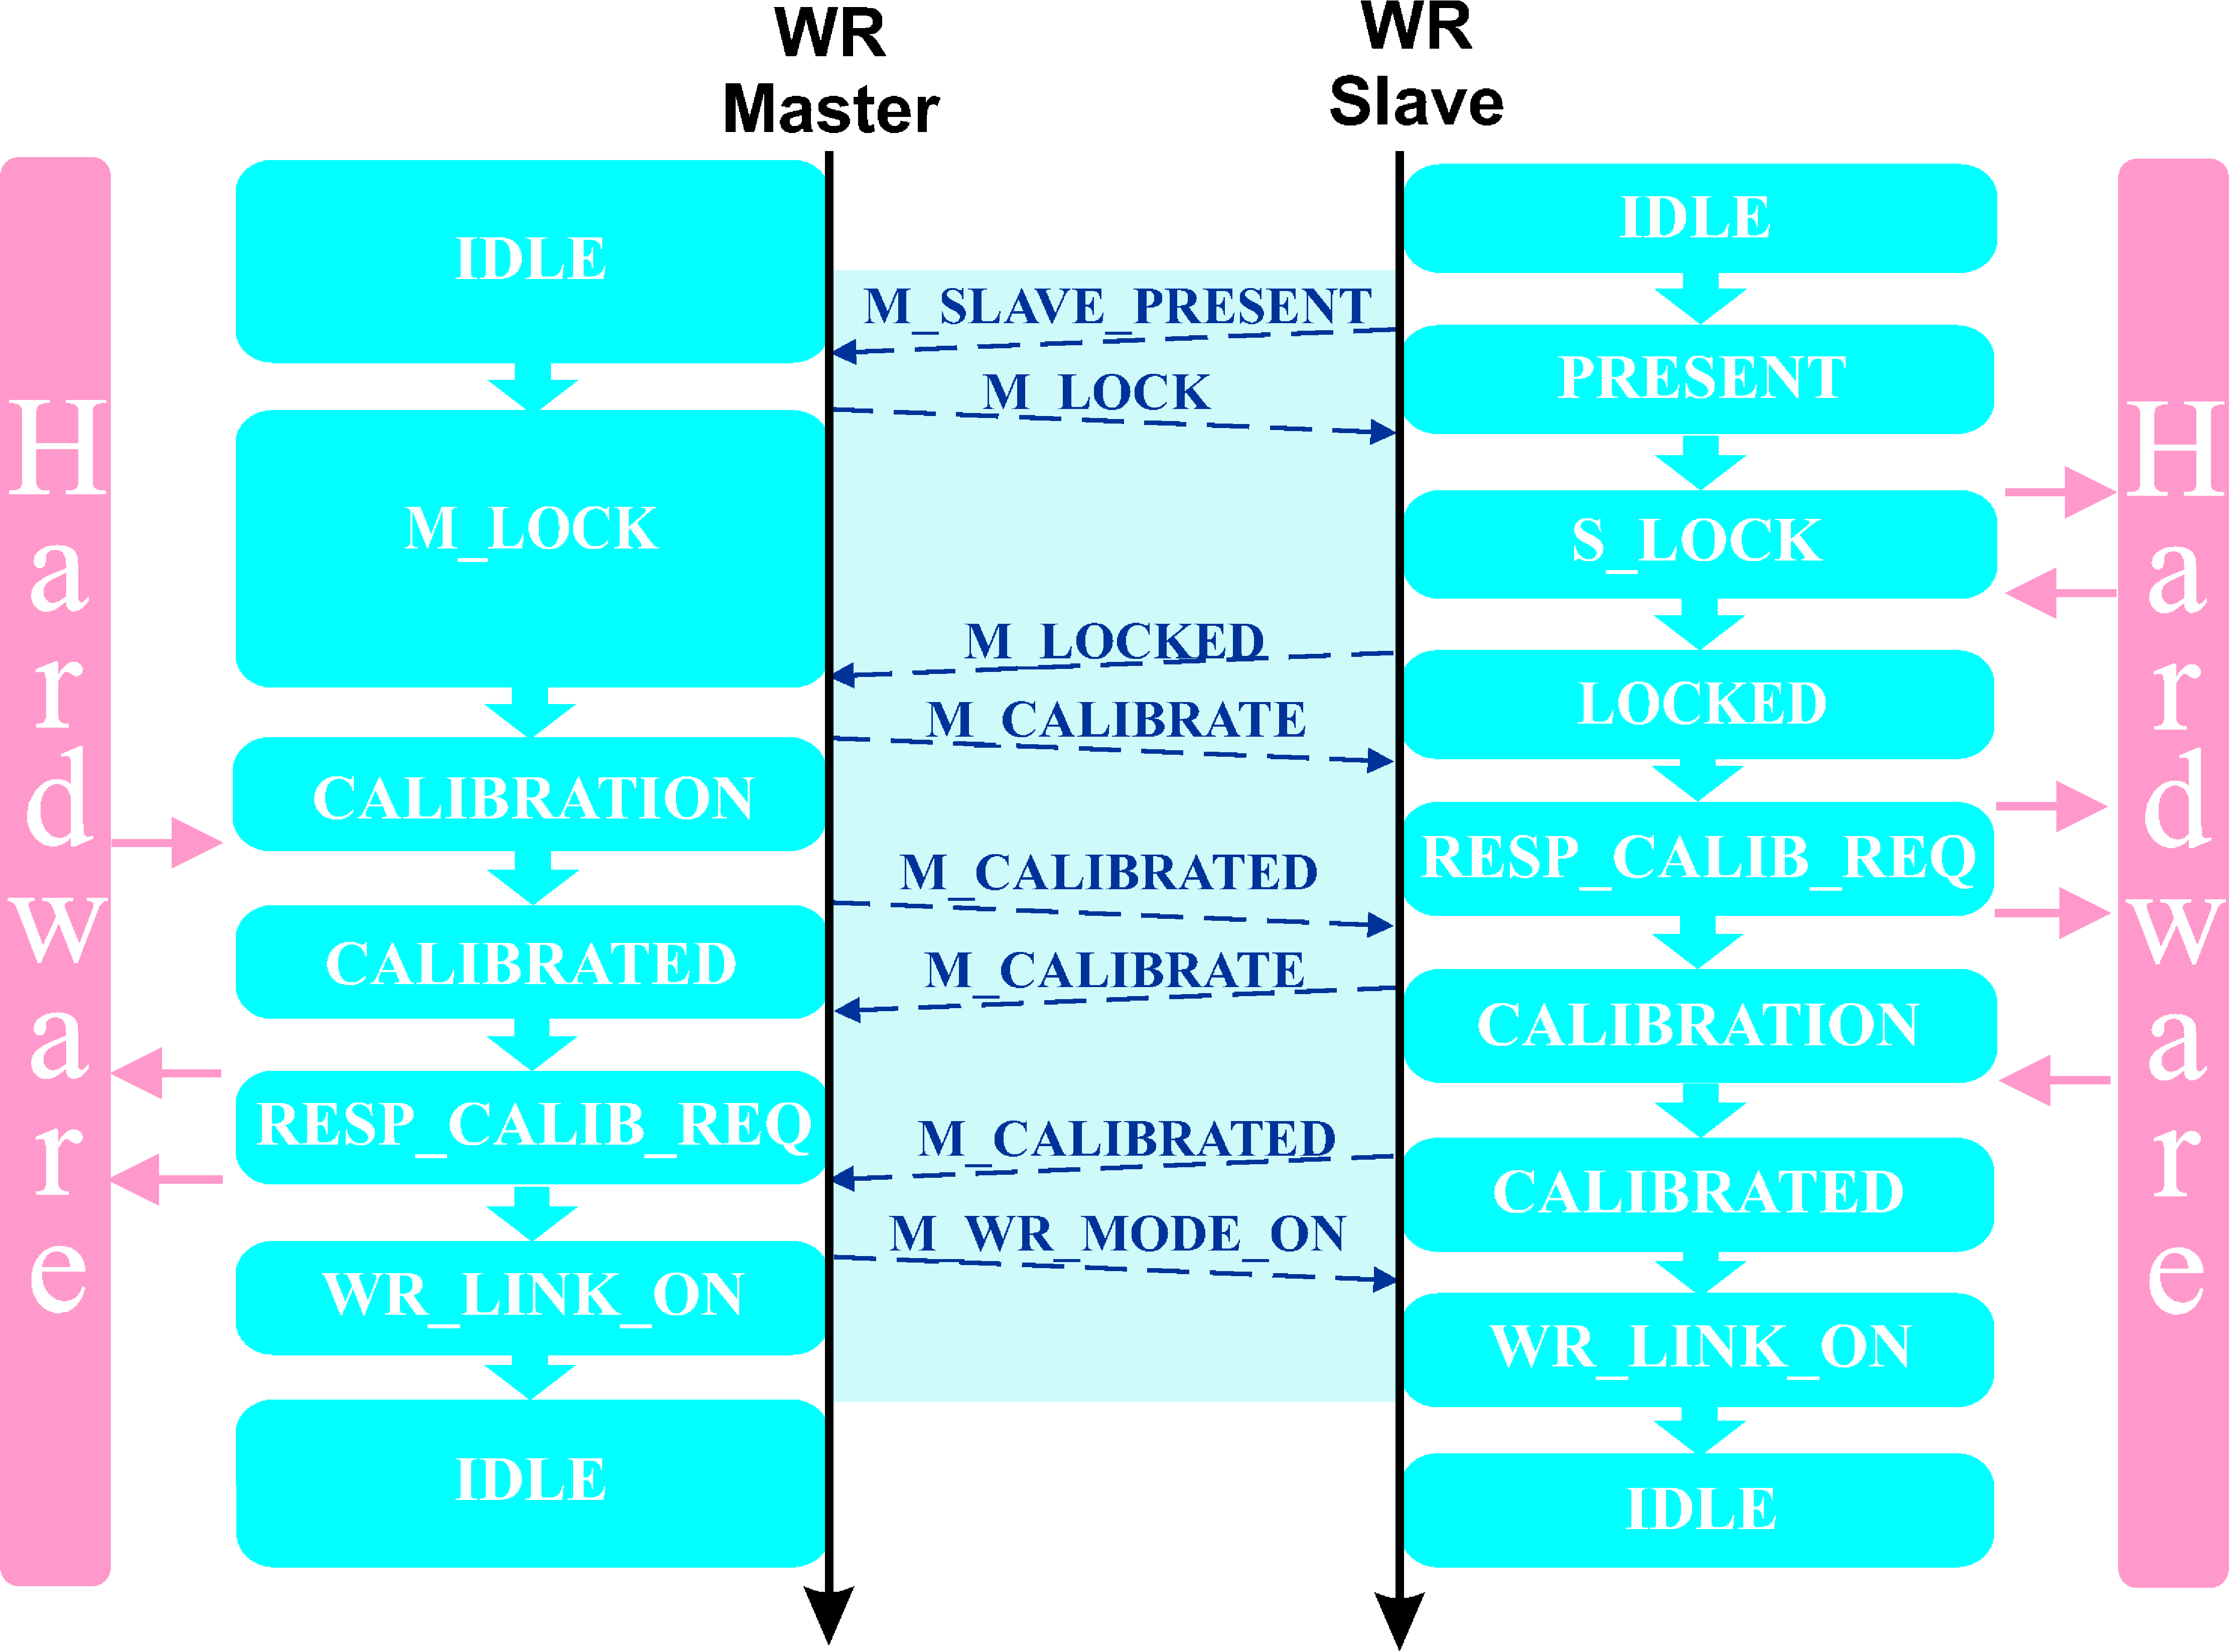
\includegraphics[width=9.5cm]{../../figures/protocol/wrLinkSetupFSM.eps}
      \end{center}

\end{frame}
%%%%%%%%%%%%%%%%%%%%%%%%%%%%%%%%%%%%%%%%%%%%%%%%%%%%%%%%%%%%%%%%%%%%%%%%%%%%%%%%%%%%%%%%%%%%%%%%%%%%
% \subsection{}
%%%%%%%%%%%%%%%%%%%%%%%%%%%%%%%%%%%%%%%%%%%%%%%%%%%%%%%%%%%%%%%%%%%%%%%%%%%%%%%%%%%%%%%%%%%%%%%%%%%%
\begin{frame}{modified BMC (mBMC)}

\begin{columns}[c]
\column{.6\textwidth}

    \begin{block}{mBMC}
    ... forces PTP\_SLAVE state instead of PTP\_PASSIVE for clockClass $>$ 127
    \end{block}

    \begin{itemize}
	\item Many PTP SLAVE ports in a single Boundary Clock
	\item Active PTP SLAVE port used to synchronize and syntonize local clock
	\item Modifies State Decision Algorithm
	\item New Data Fields update
      \end{itemize}

\column{.5\textwidth}
    \begin{center}
    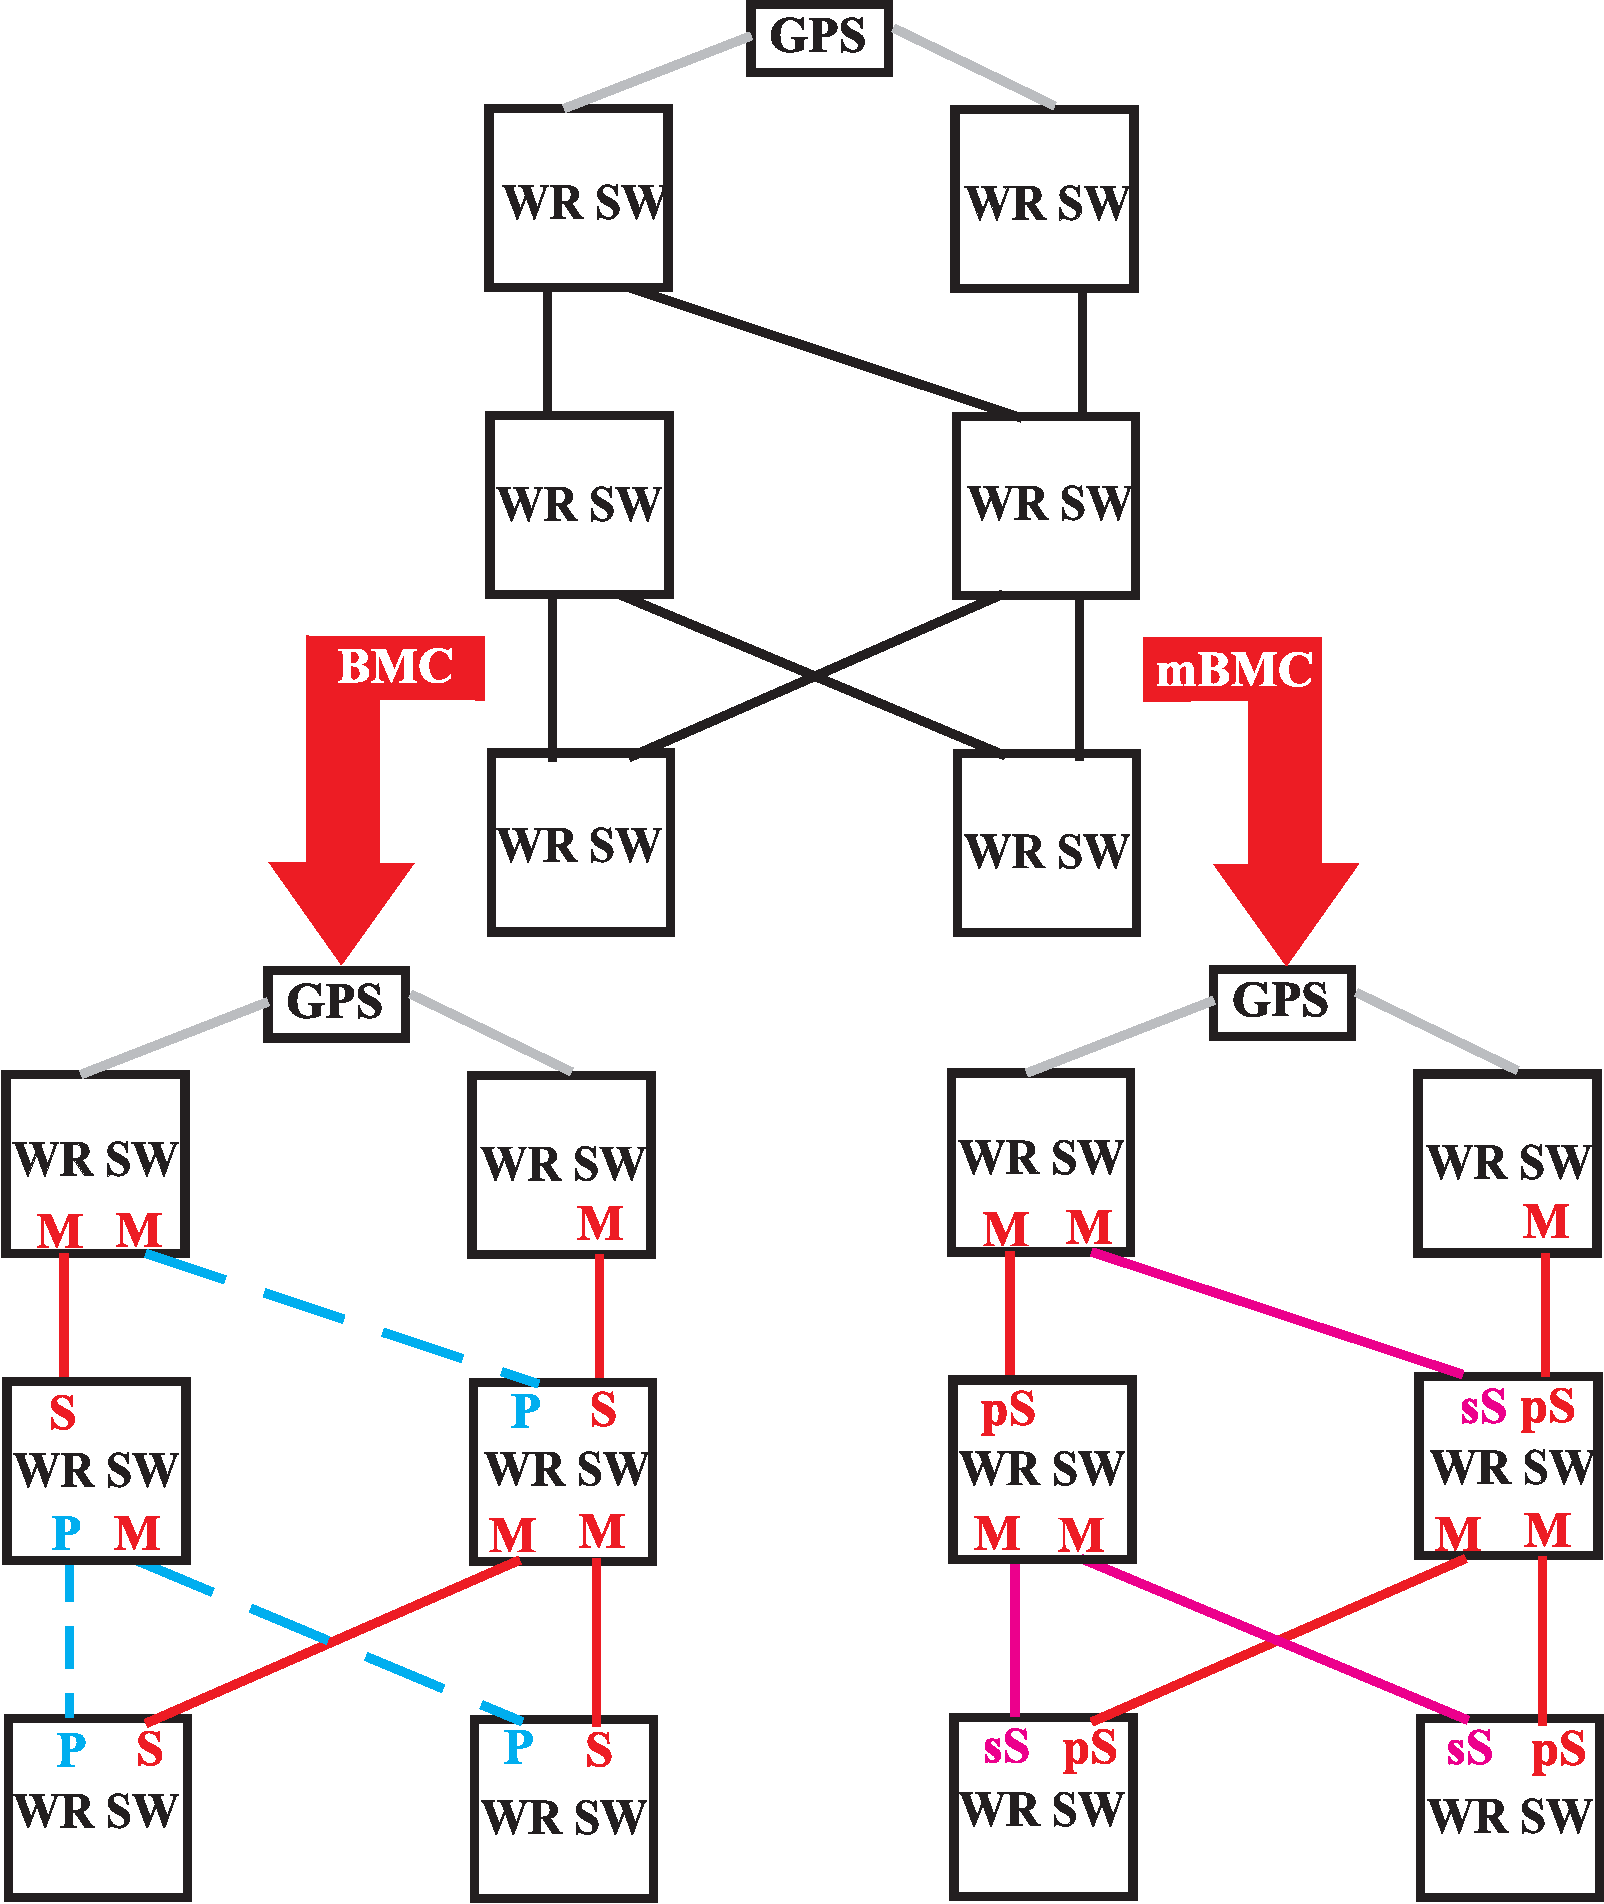
\includegraphics[height=5.5cm]{../../figures/protocol/mBMCvsBMC.eps}
    \end{center}

\end{columns}

\end{frame}
%%%%%%%%%%%%%%%%%%%%%%%%%%%%%%%%%%%%%%%%%%%%%%%%%%%%%%%%%%%%%%%%%%%%%%%%%%%%%%%%%%%%%%%%%%%%%%%%%%%%
% \section{H/W for WR}
% \subsection{H/W for WR}
%%%%%%%%%%%%%%%%%%%%%%%%%%%%%%%%%%%%%%%%%%%%%%%%%%%%%%%%%%%%%%%%%%%%%%%%%%%%%%%%%%%%%%%%%%%%%%%%%%%%
\begin{frame}{Clock Recovery System and modified BMC}

%{\it [problem with a presentation flow]}

  \begin{center}
  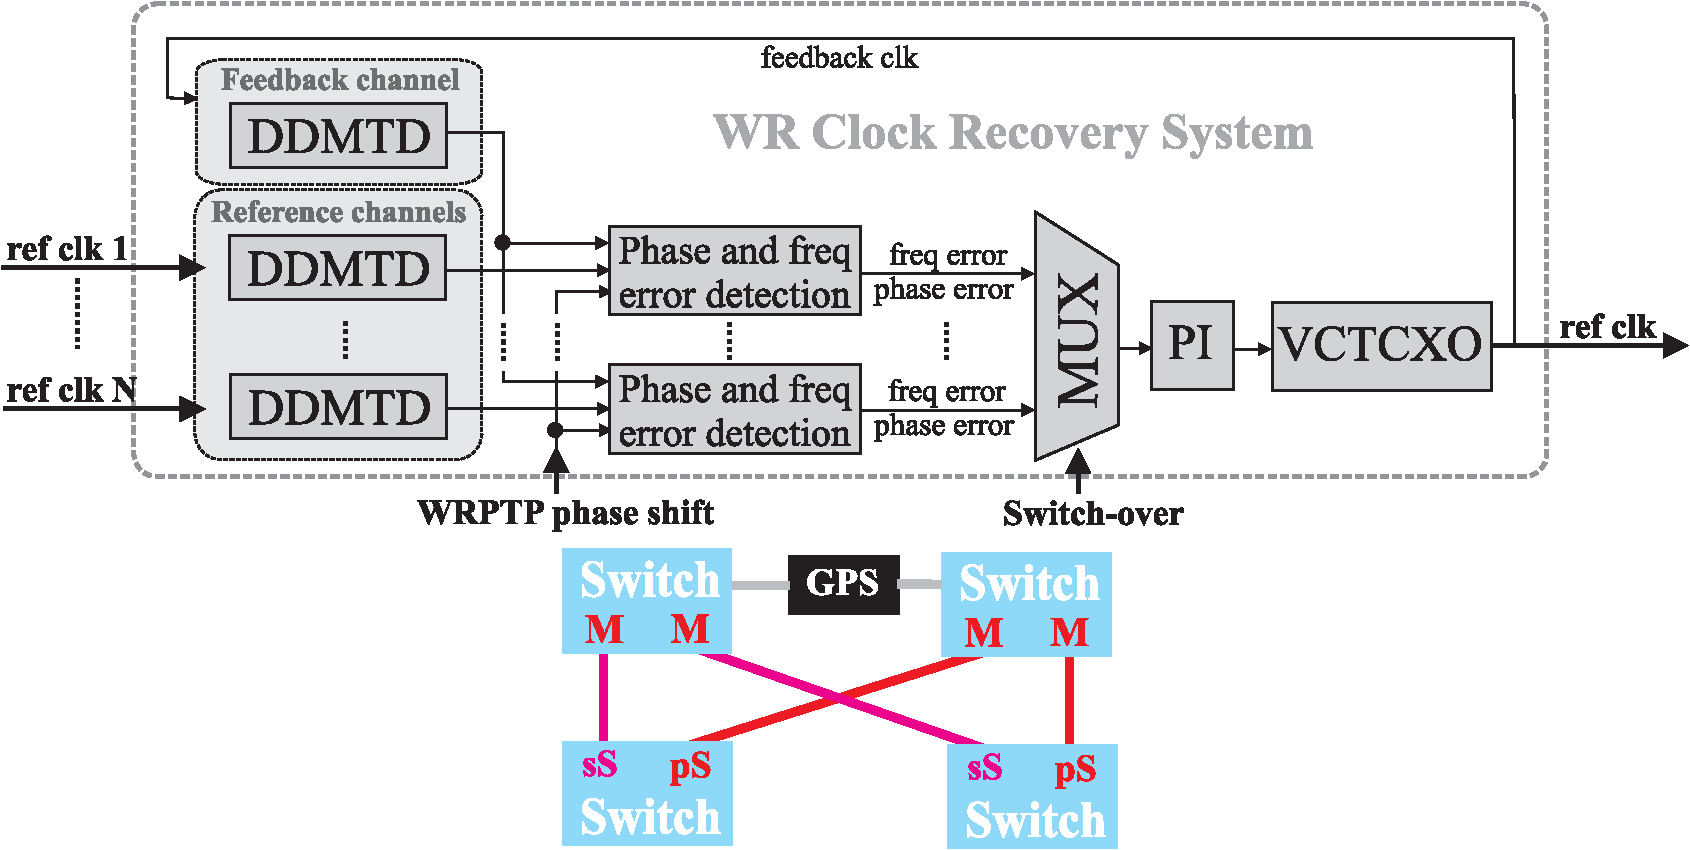
\includegraphics[width=11.8cm]{../../figures/protocol/wrCRS_plus_mBMC.eps}
  \end{center}

\end{frame}
%%%%%%%%%%%%%%%%%%%%%%%%%%%%%%%%%%%%%%%%%%%%%%%%%%%%%%%%%%%%%%%%%%%%%%%%%%%%%%%%%%%%%%%%%%%%%%%%%%%%
% \section{}
%\subsection{WRPTP Compliance}
%%%%%%%%%%%%%%%%%%%%%%%%%%%%%%%%%%%%%%%%%%%%%%%%%%%%%%%%%%%%%%%%%%%%%%%%%%%%%%%%%%%%%%%%%%%%%%%%%%%%
\begin{frame}{WRPTP profile}


\begin{columns}[c]

  \column{.17\textwidth}
  \column{.64\textwidth}

  \begin{block}{\center WRPTP profile} 
    \small 
	\begin{tabular}{| l | c |}          	     \hline
	  profle name           &  White Rabbit      \\ \hline
	  profile version       &  1.0               \\ \hline
	  profile identifier    &  08-00-03-00-01-00 \\ \hline
	  organization name     &  CERN              \\ \hline
	  source identification &  www.ohwr.org	  \\ \hline
	\end{tabular}
    \end{block}
  \column{.17\textwidth}
\end{columns}
  \vspace{0.5cm}
	\begin{tabular}{ l  l }          	     
		$->$ master clock algorighm:  & mBMC \\
		$->$ delay mechanism:         & delay request-response \\
		$->$ transport mechanism:     & IEEE 802.3 \\
		$->$ custom TLV:              & WR TLVs \\
		$->$ domain:                  & single domain only (value=0) \\
		$->$ portDS.logSyncInterval:  & default value 0, range: -1 to 6 \\
		$->$ defaultDS.priority1:     & default value 68 \\
	\end{tabular}


\end{frame}
%%%%%%%%%%%%%%%%%%%%%%%%%%%%%%%%%%%%%%%%%%%%%%%%%%%%%%%%%%%%%%%%%%%%%%%%%%%%%%%%%%%%%%%%%%%%%%%%%%%%
% \section{WRPTP requirements}
%\subsection{}
%%%%%%%%%%%%%%%%%%%%%%%%%%%%%%%%%%%%%%%%%%%%%%%%%%%%%%%%%%%%%%%%%%%%%%%%%%%%%%%%%%%%%%%%%%%%%%%%%%%%
\begin{frame}{WRPTP requirements}


% \begin{columns}[c]
%   \column{.4\textwidth}


  \begin{block}{H/W requirements}  
    \begin{itemize}
	\item SyncE
	\item Constant rx/tx latencies
	\item Support of rx/tx latencies measurement
	\item Sufficient timestamps precision
    \end{itemize}
  \end{block}

  %\column{.6\textwidth}

  \begin{block}{Implementation requirements}  
    \begin{itemize}
	\item Issue/handle WR Announce and Signaling Message
	\item non-preemptive WR Finite State Machine
	\item WR data set and WR-specific data fields
	\item SYNCHRONIZATION\_FAULT transition
	\item MASTER\_CLOCK\_SELECTED transition
	\item communication with H/W
    \end{itemize}
  \end{block}

% \end{columns}

\end{frame}
%%%%%%%%%%%%%%%%%%%%%%%%%%%%%%%%%%%%%%%%%%%%%%%%%%%%%%%%%%%%%%%%%%%%%%%%%%%%%%%%%%%%%%%%%%%%%%%%%%%%
\section{WR Spec. Changes}
\subsection{}
%%%%%%%%%%%%%%%%%%%%%%%%%%%%%%%%%%%%%%%%%%%%%%%%%%%%%%%%%%%%%%%%%%%%%%%%%%%%%%%%%%%%%%%%%%%%%%%%%%%%
\begin{frame}{Modifications}

  \resizebox{11cm}{!} 
  {
    \begin{tabular}{ r c l }
      {\bf WR Spec v1} 		& 		 & {\bf WR Spec v2}  \\
				&     		 &        \\
    WR Switch = set of ports 	& $\Rightarrow$  & WR Switch = boundary clock\\
				&      		 &        \\
    Management MSGs 	 	& $\Rightarrow$  & Signaling MSGs\\
				&      		 &        \\
    Small modificatins to 	& \multirow{2}{*}{$\Rightarrow$}   & No modifications to \\
    PTP State Machine   	&      		 & PTP State Machine       \\
				&      		 &        \\
    WR FSM in UNCALIBRATED 	& \multirow{2}{*}{$\Rightarrow$}   & WR FSM in UNCALIBRATED (Slave) \\
    (WR Master and Slave)  	&   		 & WR FSM in MASTER (Master)\\
				&      		 &        \\
    Calibration pattern:   	& \multirow{2}{*}{$\Rightarrow$}   & Calibration pattern: \\
    configurable		&      		 & RD+ K28.7      \\

    \end{tabular}
	
  }
%also modified conditions to enter WR FSM %page 33	
\end{frame}

%%%%%%%%%%%%%%%%%%%%%%%%%%%%%%%%%%%%%%%%%%%%%%%%%%%%%%%%%%%%%%%%%%%%%%%%%%%%%%%%%%%%%%%%%%%%%%%%%%%%
% \section{New addons}
% \subsection{}
%%%%%%%%%%%%%%%%%%%%%%%%%%%%%%%%%%%%%%%%%%%%%%%%%%%%%%%%%%%%%%%%%%%%%%%%%%%%%%%%%%%%%%%%%%%%%%%%%%%%
\begin{frame}{Add-ons }


   \begin{itemize}
	\item Clarity!!!
	\item HW requirements
	\item Interface with HW
	\item Modified Best Master Clock (mBMC)
	\item New Data Set and DS fields
	\item Definition of Data Set fields (re-)initialization
	\item Link Down	and re-establishing link		
	\item Specification of Tx calibration
	\item Possible knowledge of fixed delay a priori					%page 19
	\item Example implementation (Tomek's MSc)
	\item WR computations
	\item WRPTP Profile \& Requirements

%	\item Definition of boundary clock, ordinary clock 					%page 16

%	\item Clarification of when Signaling Messages are sent/received 	%page 28
%	\item Definition of PTP FSM implementation-specific transitions 	%page 31
%	\item Communication between WR State Machines						%page 38
%	\item Communication between WR State Machine and HW					%page 39
					%page 41
%	\item Specification of re-try mechanism
%	\item Definition of Link Down and Link re-establishing

   \end{itemize}

\end{frame}

%%%%%%%%%%%%%%%%%%%%%%%%%%%%%%%%%%%%%%%%%%%%%%%%%%%%%%%%%%%%%%%%%%%%%%%%%%%%%%%%%%%%%%%%%%%%%%%%%%%%
\section{Conclusions}
\subsection{}
%%%%%%%%%%%%%%%%%%%%%%%%%%%%%%%%%%%%%%%%%%%%%%%%%%%%%%%%%%%%%%%%%%%%%%%%%%%%%%%%%%%%%%%%%%%%%%%%%%%%
\begin{frame}{Improvements and Conclusions}

\begin{itemize}
  \item Great feedback from John Eidson
  \item Thicker but clearer
  \item NO changes to PTP standard (v1 included a few)
  \item WR Switch became a full-blown Boundary Clock!!!
  \item Better fitted for standardization attempts
%   \item ISPCS2011: possible joined efforts with Frence Telecom in standardization (!?)
\end{itemize}

\end{frame}
%%%%%%%%%%%%%%%%%%%%%%%%%%%%%%%%%%%%%%%%%%%%%%%%%%%%%%%%%%%%%%%%%%%%%%%%%%%%%%%%%%%%%%%%%%%%%%%%%%%%
\section{}
%\subsection{}
%%%%%%%%%%%%%%%%%%%%%%%%%%%%%%%%%%%%%%%%%%%%%%%%%%%%%%%%%%%%%%%%%%%%%%%%%%%%%%%%%%%%%%%%%%%%%%%%%%%%
\begin{frame}{thank you}

    \begin{center}
    Any questions ?
    \end{center}

    
    \begin{center}
%    \includegraphics[height=4.0cm]{fig/white_rabbit_by_kyoht.ps}
%    \includegraphics[height=4.0cm]{fig/WRlogo.ps}
    
\includegraphics[height=3.0cm]{../../figures/misc/white_rabbit_end.eps}
    \end{center}

\end{frame}
%%%%%%%%%%%%%%%%%%%%%%%%%%%%%%%%%%%%%%%%%%%%%%%%%%%%%%%%%%%%%%%%%%%%%%%%%%%%%%%%%%%%%%%%%%%%%%%%%%%%



\end{document}
